\documentclass{book}
\usepackage[utf8]{inputenc}
\usepackage{amsmath}
\usepackage{mathrsfs}
\usepackage{float}
\usepackage[margin = 1.5in]{geometry}

\usepackage{xcolor}
\usepackage{pdflscape}
\usepackage{url}
\usepackage{nameref}
\title{\textbf{dismolib}\\
COPASI-based infectious disease models library}
\author{}
\date{Last updated: August 2021}

\usepackage{natbib}
\usepackage{graphicx}

\usepackage{color}   %May be necessary if you want to color links
\usepackage{hyperref}
\hypersetup{
    colorlinks=true, %set true if you want colored links
    linktoc=all,     %set to all if you want both sections and subsections linked
    linkcolor=blue,  %choose some color if you want links to stand out
}

\newcommand{\blue}[1]{{\textcolor{blue}{#1}}}

\begin{document}

\maketitle

\tableofcontents

\chapter{Introduction}
\label{chapt:intro}

% https://www.overleaf.com/project/5f70b98896d4f90001617491
%``The basic reproductive number is often treated as a biologically determined characteristic of the pathogen’s transmissibility, it is actually a combination of biological, environmental, behavioral, and social characteristics, including relative transmissibility via different pathways'', \cite{eubank2020commentary}.

We have compiled a set of compartmental deterministic models for transmissible diseases, ready for use in the COPASI Biochemical System Simulator software (and other SBML standard compliant tools). Models were chosen to represent globally relevant diseases, as well as a diversity of disease types and infection mechanisms. These models aim to exemplify commonly used mathematical analyses, as well as numerical simulations, using COPASI. A primary goal is to provide inexperienced users an amenable introduction to the basics of mathematical modeling of infectious diseases. Provided examples show how one can formulate and numerically explore and analyze a mathematical models. We also aim to promote consistency between modeling efforts by making it easier to use existing standards. This should save people time and effort by enabling them to build from pre-existing models, as well as foster collaboration and reproduceability.

In the sections to follow, we will study basic mathematical models for selected diseases. Chapters \ref{chapt:waterborne} through \ref{chapt:vectorborne} consider diseases by mechanism of infection: water-borne diseases, sexually-transmitted diseases, airborne diseases and vector-borne diseases. Each of these chapters considers each disease case in terms of its epidemiology, a model extracted from literature, a short mathematical analysis, and the COPASI-related code. The following points will be addressed, as relevant for each disease case. These will ultimately relate to specifics in the COPASI model structure and simulation settings.

\begin{enumerate}
    \item Infection mechanism (E.g. seasonality)
    \item Transmission agents (human, vector, animal host, animal reservoir, environment like water bodies, soil, etc.)
    \item Mixing structure (homogeneous, age-structured, sex-structured, spatial metapopulation)
    \item Region
    \item Interventions (Vaccination, social distancing, preventative and curative treatment)
    \item Initial conditions (based on the research question) and temporal changes in the interventions (e.g. vaccination is one time phenomenon whereas social distancing may vary over time)
\end{enumerate}

The \nameref{chapt:genmods} chapter (\ref{chapt:genmods}) covers slight modifications of the presented models. Chapter (\ref{chapt:finsize}), \nameref{chapt:finsize}, looks at techniques used to compute the final epidemic size of various models. 

%\textcolor{purple}{Smriti's comment: Just a thought, would adding another characteristic like being a communicable disease and a noncommunicable disease, would be relevant to the study?} \textcolor{red}{MT: All of the diseases considered are communicable since we are modeling the transmission process at a population level for now}

The COPASI files for the following models and reproduced results from the respective referenced papers and can be found at \url{https://github.com/mugdhat2/CopasiDiseaseLibrary}.


\chapter{Water-borne Diseases}
\label{chapt:waterborne}

\section{Cholera}
%\textcolor{red}{Needs paraphrasing to be publishable}
\subsection*{Introduction}
Cholera is an acute, diarrheal illness caused by infection of the intestine with the toxigenic bacterium {\it Vibrio cholerae}. It is estimated Cholera is responsible for 2.9 million cases and 95,000 deaths annually worldwide. The infection is often mild or without symptoms, but can be severe. Approximately 1 in 10 people who get sick with cholera will develop severe symptoms such as watery diarrhea, vomiting, and leg cramps. In these people, rapid loss of body fluids leads to dehydration and shock. Without treatment, death can occur within hours.

A person can get cholera by drinking water or eating food contaminated with cholera bacteria. In an epidemic, the source of the contamination is usually the feces of an infected person that contaminates water or food.

\subsection*{Mathematical Model}
Assume the health stages Susceptible ($S$), Infected ($I$) and Recovered ($R$), and let $B$ denote the concentration of vibrios in contaminated water. The following \cite{sun2017transmission}, two transmission paths for Cholera are considered: environment-to-human transmission and human-to-human transmission.

Susceptible individuals are assumed to be recruited proportionally to the population size, $\mu N$, and can become infected by drinking contaminated water at rate $\beta_{e}\frac{B}{k+B}$, or by contact with infected individuals at rate $\beta_{h}I$. In addition, susceptible individuals might get vaccinated and become permanently immune at rate $\nu$, or die at rate $\mu$.
Infected individuals are assumed to permanently recover on average after $\frac{1}{\gamma}$ days or die at rate $\mu$.
Contaminated water is assumed to be generated by infected individuals at rate $\xi$, and it cleans up by natural vibrios decayment at rate $\delta$ or by disinfection at rate $c$.

\begin{figure}
    \centering
    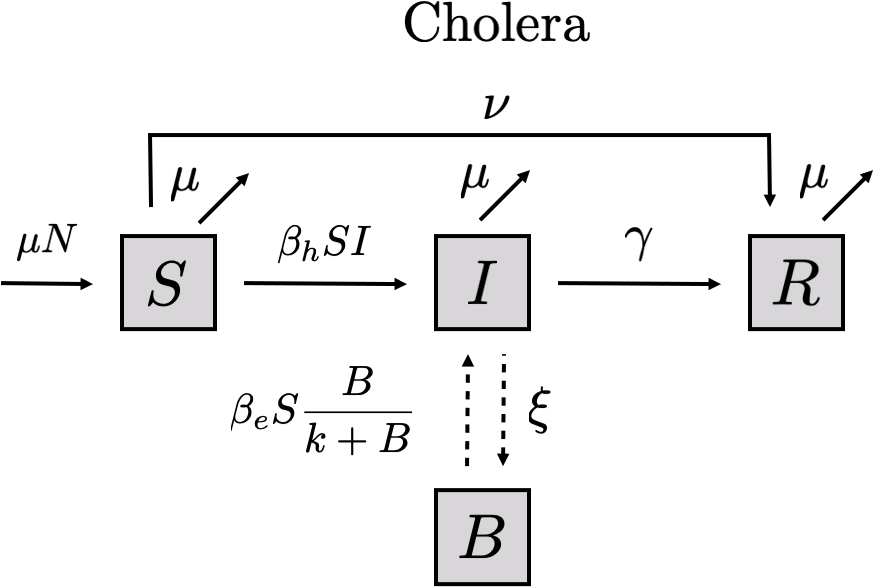
\includegraphics[width = 0.6\textwidth]{Flowcharts/cholera.png}
    \caption{Flowchart of Cholera disease model}
    \label{fig:cholera_flow}
\end{figure}

The aforementioned disease dynamics are captured in the following system of Ordinary Differential Equations (ODE).
%
\begin{equation} \label{eq:cholera_model}
\left\{\begin{array}{l}
\frac{d S}{d t}=\mu N-\left(\beta_{e} S \frac{B}{k+B}+\beta_{h} S I\right)-\mu S-v S \\
\frac{d I}{d t}=\beta_{e} S \frac{B}{k+B}+\beta_{h} S I-(\gamma+\mu) I \\
\frac{d R}{d t}=\gamma I-\mu R+v S \\
\frac{d B}{d t}=\xi I-\delta B-c B
\end{array}\right.
\end{equation}
%
where $\mu$ represents natural birth or death rate, $N(S+I+R=N)$ denotes the total population in China, $k$ corresponds to the concentration of vibrios in contaminated water, $\xi$ is the rate of human contribution to vibrio Cholera, $\delta$ is the decay rate of vibrios 

With estimated parameters $\beta_e=a\times 10^{-6}$, $\beta_h=b\times 10^{-9}$ and $\nu$.
%
\subsection*{Model Analysis}
The presented mathematical model incorporates population dynamics that allow the model to reach an endemic level (non-zero steady state) in the population.
In the absence of cholera, model \eqref{eq:cholera_model}, assumes a constant total population since
$$
\frac{d N}{d t}=\frac{d S}{d t}+\frac{d I}{d t}+\frac{d R}{d t}=0
$$
Therefore, it is enough to consider the following equations
\begin{equation} \label{eq:reduced_cholera}
\begin{aligned}
\frac{d S}{d t} &=\mu N-\beta_{e} S \frac{B}{k+B}-\beta_{h} S I-\mu S-v S \\
\frac{d I}{d t} &=\beta_{e} S \frac{B}{k+B}+\beta_{h} S I-(\gamma+\mu) I \\
\frac{d B}{d t} &=\xi I-\delta B-c B
\end{aligned}
\end{equation}
%
Making system \eqref{eq:reduced_cholera} equal to zero, and solving for the population variables, we get the disease-free equilibrium (DFE) under control policies (vaccination)
\begin{equation}
E_{0}=\left(\frac{\mu N}{\mu+v}, 0,0\right)
\end{equation}
and the following endemic equilibrium
$$
E^{*}=\left(S^{*}, I^{*}, B^{*}\right), \text { where } I^{*}=\frac{(\delta+c) B^{*}}{\xi} \text { and } S^{*}=\frac{\mu N \xi-(\gamma+\mu)(\delta+c) B^{*}}{(\mu+v) \xi}
$$
Following the Next Generation Matrix (NGM) approach with infectious compartments $I$ and $B$, the control reproductive number of system \eqref{eq:cholera_model} is given by
%\textcolor{purple}{Brian's comment: Is "the next generation approach" a formal concept? If so, it should be somehow indicated with capitalization, or something.}
\begin{equation}
\mathcal{R}_C=\mathcal{R}_h+\mathcal{R}_e=\beta_{h} \frac{\mu N}{(\mu+v)(\gamma+\mu)}+\beta_{e} \frac{\mu N \xi}{(\mu+v)(\gamma+\mu)(\delta+c) k}
\end{equation}
which collects the secondary infections produced by infected individuals during its infectious period $\frac{1}{\gamma+\mu}$ at rate $\beta_h$ and, the secondary infections produced by contaminated water at rate $\beta_e \frac{\xi}{\kappa}$ during its contamination period $\frac{1}{\delta+c}$, generated by infected individuals during their infectious period $\frac{1}{\gamma+\mu}$, in a partially susceptible population $S_0=\frac{\mu N}{\mu+\nu}$.

Notice that the control reproductive number $\mathcal{R}_C$, reduces to the basic reproductive number $\mathcal{R}_0$, in the absence of vaccination. In this case, $S_0=N$ and the basic reproductive number is given by

    \begin{equation}
    \mathcal{R}_0=N\left(\beta_{h} \frac{ 1}{(\gamma+\mu)}+\beta_{e} \frac{ \xi}{(\gamma+\mu)(\delta+c) k}\right)
\end{equation}

\subsection*{Simulations}
To simulate the model we use the parameters in Figure \ref{fig:cholera_pars}.

%\textcolor{red}{Initial conditions missing. It would be preferable for the units to be consistent. Rewrite parameter estimate table with final values.}
%
\begin{figure}[H]
    \centering
    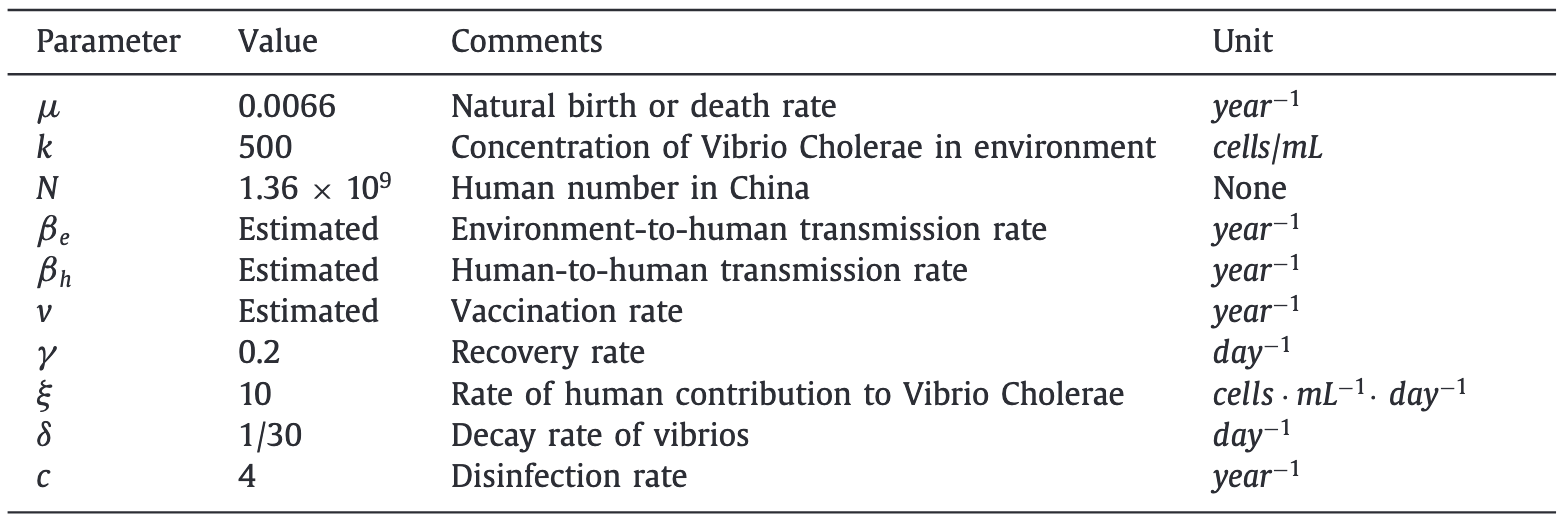
\includegraphics[scale=0.35]{cholera1}
    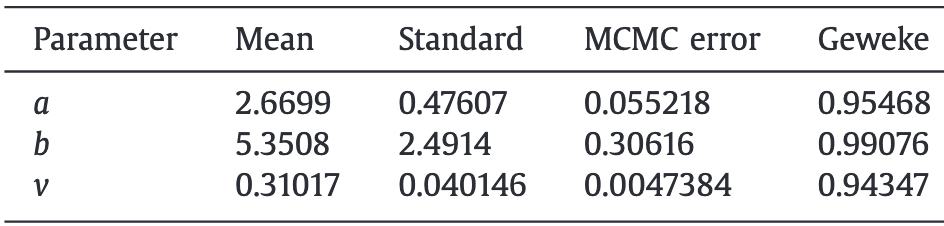
\includegraphics[scale=0.35]{cholera2}
    \caption{Parameters for Cholera model}
    \label{fig:cholera_pars}
\end{figure}

\subsection*{Model Remarks}
The studied cholera model incorporates several key components: 
%
(i) due to the endemic nature of cholera in the affected regions, a model with demographic processes is used;
%
(ii) the water and human based cholera transmission routes require addressing both infection forces in order to appropriately capture disease dynamics and thresholds;
%
(iii) the availability of vaccine makes it important to study cholera dynamics in the absence and in the presence of control measures (vaccination): (a) cholera dynamics in a completely susceptible population and, (b) cholera dynamics in a partially susceptible population, for which disease dynamics exhibit, the basic reproductive number and the control reproductive number (disease eradication via control measures), $\mathcal{R}_0$ and $\mathcal{R}_C$ respectively.

Finally, notice that $\mathcal{R}_C$ and $\mathcal{R}_0$ of model \eqref{eq:cholera_model}, are directly proportional to the population size. This is due to the mass action formulation $\beta SI$, as opposed to the standard incidence formulation $\beta S \frac{I}{N}$. The fact that the basic and the control reproduction numbers are functions of the population size, has direct implications to public health policies.

\begin{table}[]
    \centering
    \begin{tabular}{|l|l|} \hline
      Disease   & Cholera \\ \hline
         Transmission pathway(s)& 
         \begin{tabular}{l}
             - Human-to-human \\
             - Water-to-human 
         \end{tabular}\\ \hline
         Intervention Scenarios & 
         \begin{tabular}{l}
             - No Intervention \\
             - Disinfection of water (at rate $c$)\\
             - Vaccination (at rate $\nu$)
         \end{tabular}\\ \hline
         Model source & \cite{sun2017transmission}\\ \hline
         Unique modeling aspect & Simple model with 
         \begin{tabular}{l}
           - environmental transmission mode     \\
           - vaccination   
         \end{tabular} \\ \hline
         Location & China\\ \hline
         Initial conditions & $I_0 =28$; $B_0 = 500$ (Assumed$^*$)\\ \hline
         Parameter estimate remarks & \begin{tabular}{l}
            - Sources of parameter estimates not given  \\
            - For $R_0<1$, Figure 5 shows positive equilibrium\\
            - Same data used to fit and validate the model %(\textcolor{red}{verify})
         \end{tabular}\\ \hline
         Data Sources & NA \\  \hline
         Reproducibility remarks & Figures 5 and 6 reproduced\\ \hline
         Possible extensions & \begin{tabular}{l}
            -  Waning immunity upon recovery and vaccination \\
            - Finer spatial resolution
         \end{tabular} \\ \hline
         
    \end{tabular}
    \caption{Cholera: Summary and reproducibility attributes. $^*$ Information missing in paper}
    \label{tab:cholera_summary}
\end{table}
%\section{Hepatitis}

\section{Typhoid}
\subsection*{Introduction}
\subsection*{Mathematical model}
Following the work in \cite{peter2017mathematical}, we assume the population under study is subdivided in the following health classes: Susceptible individuals ($S$), Infected and infectious individuals ($I$), Infected and not infectious individuals due to treatment ($T$), and Recovered individuals ($R$). The model also assumes that some susceptible individuals are vaccinated and loss immunity after a period of time ($P$).

\begin{figure}[H]
    \centering
    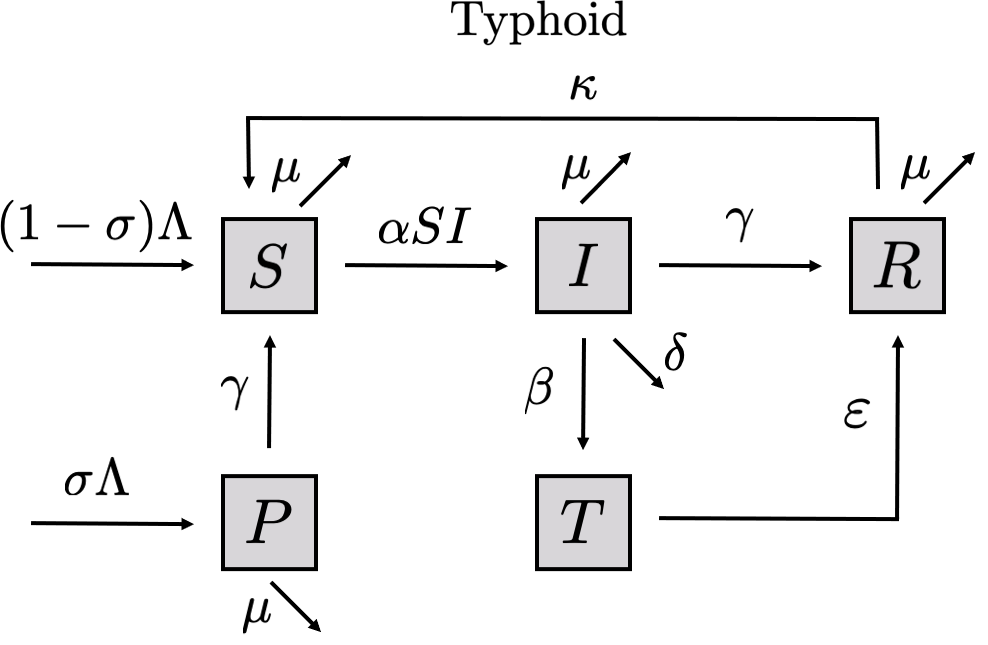
\includegraphics[width = 0.6\textwidth]{Flowcharts/typhoid.png}
    \caption{Flowchart of Typhoid disease model}
    \label{fig:typhoid_flow}
\end{figure}

The proposed model assumes that susceptible individuals are being recruited at a constant rate $\Lambda$ and die at a per-capita rate $\mu$.

The fraction $\sigma$ of recruited susceptible individuals are assumed to be vaccinated, becoming temporary protected against Typhoid on average for a period of $\frac{1}{\gamma}$. The fraction of non-vaccinated recruited individuals $1-\sigma$ becomes susceptible. Typhoid is transmitted by contacts between infected and susceptible individuals at a rate $\alpha S I$. 
%
Infected individuals either, undergo disease-induced death at a rate $\delta I$, go to treatment at a rate $\beta I$, or die by other reasons at a per-capita rate $\mu$.
%
Individuals under treatment recover at a per-capita rate $\epsilon$, loosing natural immunity at a per-capita rate $\kappa$, or die out by other reasons at a per-capita rate $\mu$.
%

\begin{equation}
\begin{array}{l}
\frac{d P}{d t}=\sigma \Lambda-(\gamma+\mu) P \\
\frac{d S}{d t}=(1-\sigma) \Lambda+\gamma P-\alpha S I-\mu S+k R \\
\frac{d I}{d t}=\alpha S I-(\delta+\beta+\mu) I \\
\frac{d T}{d t}=\beta I-(\mu+\varepsilon) T \\
\frac{d R}{d t}=\varepsilon T-\mu R-k R
\end{array}
\end{equation}

\subsection*{Model Analysis}
\subsection*{Simulations}
Assumptions:
\begin{itemize}
    \item $I$ (Infectious individuals) in the coded model is equivalent to $I_e$ (educated infectious individuals) in \cite{akinduko2018series} since the models closely resemble.
    \item $(P_0, S_0, I_0, T_0, R_0)$ = $(100, 200, 120, 80,60)$ based on Figures in \cite{akinduko2018series}
    \item Parameter estimation from \cite{akinduko2018series} as shown in Table \ref{tab:typhoid_params}
\end{itemize}

\begin{table}[]
    \centering
    \begin{tabular}{c l c c}\hline
        Parameter & Definition & Assumption from \cite{akinduko2018series} & Value  \\ \hline
         $\alpha$ & Infection transmission coefficient & $\beta_2$ & 0.05\\
         $\beta$ & Treatment initiation rate & $\phi_2$ & 0.3\\
         $\delta$ & Disease induced mortality rate & $\delta$ & 0.075\\
         $\epsilon$ & Recovery rate & $\epsilon$ & 0.4\\
         $\gamma$ & Rate of waning immunity of protected individuals & $\omega$ & 0.5\\
         $k$ & Immunity waning rate of recovered individuals & $0$ & 0\\
         $\Lambda$ &Total recruitment rate of individuals & $\Lambda$ & 200\\
         $\mu$ & Natural mortality rate & $\mu$ & 0.142\\
         $\sigma$ & Vaccination proportion & $\tau/\Lambda$ &0.092\\ \hline
    \end{tabular}
    \caption{Parameter estimates adapted from \cite{akinduko2018series}. Time units in decades. }
    \label{tab:typhoid_params}
\end{table}



\begin{table}[]
    \centering
    \begin{tabular}{|l|p{4in}|} \hline
      Disease   &  Typhoid\\ \hline
         Transmission pathway(s)& Human-to-human\\ \hline
         Intervention Scenarios & 
         \begin{tabular}{l}
              - No Intervention \\
              - Treatment \\
              - Vaccination
         \end{tabular}\\ \hline
         Model source & \cite{peter2017mathematical}\\ \hline
         Unique modeling aspect & \begin{tabular}{p{4in}}
              - Capturing water-borne transmission without an explicit class for contaminated water\\
              - Waning immunity of vaccination captured  \\
              - Individuals in treatment are not infectious
         \end{tabular}\\ \hline
         Location & Non-specific\\ \hline
         Initial conditions & Assumed based on Figures in \cite{akinduko2018series}\\ \hline
         Parameter estimate remarks & Assumed based on estimates in \cite{akinduko2018series}\\ \hline
         Data Sources & NA\\ \hline
         Reproducibility remarks & Simulations approximate Figures 2, 3, 5, 6 and 7 in \cite{akinduko2018series}\\ \hline
         Possible extensions & Transmission pathway through contaminated food and water\\ \hline
         
    \end{tabular}
    \caption{Typhoid: Summary and reproducibility attributes}
    \label{tab:typhoid_summary}
\end{table}
\subsection*{Model remarks}
The proposed model assumes a mass action law in the non-linear term ($\alpha S I$), which assumes that every susceptible individual makes contacts with every infected individual. This assumption may be appropriate in the case of small populations, but inaccurate as the total population size increases.
%
A direct consequence of the mass-action assumption is that the basic reproductive number is proportional to the population size. In other words, the model assumes that the number of secondary cases produced by a single infected individual increases as the population size increases.

\section{Dysentery}

\subsection*{Introduction}
Dysentery can result from bacteria, virus or parasitic infection. It is commonly caused by shigella dysenteriae serotype 1 (bacillary dysentery) or Entamoeba histolytica (amoebic dysentery). Without adequate hydration, it can be fatal.

Although preventable and treatable, it is common worldwide. Dysentery epidemics regularly occur in less developed areas of Central and South America, Africa, and Asia. It tends to be a major problem among refugee populations, where overcrowding and poor sanitation facilitate transmission.

\subsection*{Mathematical model}

Based on the work by Weldegiorgis et.al. \cite{berhe2019parameter}, the population of interest is subdivided into Susceptible ($S$), Infected ($I$) and Recovered ($R$) individuals. The infectious pathogen is denoted by $B$.

\begin{figure}[H]
    \centering
    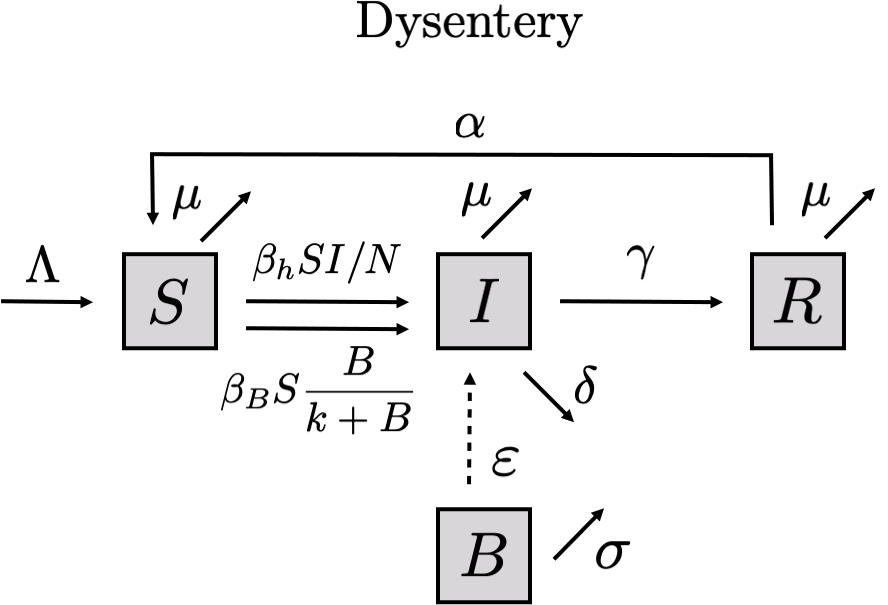
\includegraphics[width = 0.6\textwidth]{Flowcharts/dysentery.png}
    \caption{Flowchart of Dysentery disease model}
    \label{fig:dysentery_flow}
\end{figure}

The proposed model assumes susceptible individuals are recruited at a constant rate $\Lambda$, and assumes individuals die out at the per-capita rate $\mu$, regardless of their health status. 
%
Susceptible individuals are assumed to become infected by contact with infectious individuals $\left(\lambda_h=\beta_{h}\frac{I}{N}\right)$ or by ingesting the infectious pathogen $\left(\lambda_B=\beta_{B}\frac{B}{K+B} \right)$, where $\beta_B$ represents the rate of ingesting the pathogen from the contaminated environment, and $\beta_h$ through human to human interaction.
%
The infection due to virus ingestion is assumed to follow a logistic shape, where the 50\% chance of acquiring the infection is denoted by $K$.
%
Infected individuals recover at a per-capita rate $\gamma$ or die from natural causes or by disease-induced deaths at a per-capita rate $d$.
%
Recovered individuals die out or are assumed temporarily immune, before becoming susceptible again at a rate $\alpha$.
%
The infectious pathogen is assumed to be shed by infectious individuals at a rate $\epsilon I$, and it is assumed the pathogen clears at a rate $\sigma$.

The dynamics of disease progression among individuals in the affected population is described by the following system of ODE's

\begin{equation}
\begin{array}{l}
\frac{d S}{d t}=\Lambda+\alpha R-\left(\lambda_{h}+\lambda_{B}+\mu\right) S \\
\frac{d I}{d t}=\left(\lambda_{h}+\lambda_{B}\right) S-(\mu+\gamma+d) I \\
\frac{d R}{d t}=\gamma I-(\mu+\alpha) R \\
\frac{d B}{d t}=\epsilon I-\sigma B
\end{array}
\end{equation}
where
\begin{equation}
\lambda_{h} =\beta_{h}\frac{I}{N} \text { and } \lambda_{B} =\beta_{B}\frac{B}{K+B}
\end{equation}

\subsection*{Model analysis}
Notice that the population is not constant and therefore we start computing the population's steady state. The population size is governed by the equation
$\frac{dN}{dt}=\Lambda -\mu N$,
with a steady state $N^*=\frac{\Lambda}{\mu}$.
Therefore the disease-free equilibrium is given by 
\begin{equation}
E^*=\left(\frac{\Lambda}{\mu},0,0 \right).
\end{equation}

Using the next generation approach with the infectious compartments $I$ and $B$, we get the basic reproductive number
\begin{equation}
R_{0}=\frac{\beta_{h}}{(\mu+\gamma+d)}+\frac{\Lambda \beta_{B} \epsilon}{\mu(\mu+\gamma+d) K \sigma}
\end{equation}
which accounts for the average number of secondary infections produced by a single infected individual $\left( \frac{\beta_{h}}{\mu+\gamma+d} \right)$, and the average infections produced by the infected environment.
\subsection*{Simulations}
\begin{table}[ht]
    \centering
    \begin{tabular}{|l|l|} \hline
      Disease   & Dysentery \\ \hline
         Transmission pathway(s)& \begin{tabular}{l}
             - Human-to-human  \\
             - Water-to-human 
         \end{tabular}\\ \hline
         Intervention Scenarios & 
         \begin{tabular}{l}
             - No Intervention \\
              
         \end{tabular}\\ \hline
         Model source & \cite{berhe2019parameter}\\ \hline
         Unique modeling aspect & Waning immunity of recovered people\\ \hline
         Location & Ethiopia\\ \hline
         Initial conditions & \begin{tabular}{l}
              - Values used from Table 3 in \cite{berhe2019parameter}  \\
              - $I_0$ differs in Table 3 and Figure 4 in \cite{berhe2019parameter}
         \end{tabular}\\ \hline
         Parameter estimate remarks & Time course for given parameters does not fit the data\\ \hline
         Data Sources & Table 2 in \cite{berhe2019parameter}\\ \hline
         Reproducibility remarks & Figure 4 in \cite{berhe2019parameter} reproducible for $K = 28158$, $\alpha = 0.14$, $\gamma = 0.124$\\ \hline
         Possible extensions & Age-structure model since children are at most risk\\ \hline
         
    \end{tabular}
    \caption{Dysentery: Summary and Reproducibility attributes}
    \label{tab:dysentery_params}
\end{table}
%
\begin{figure}[ht]
    \centering
    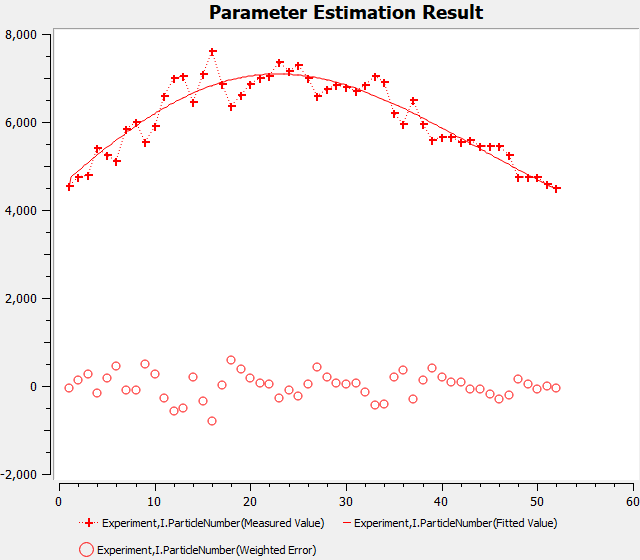
\includegraphics[width = 0.6\textwidth]{ModelFit.png}
    \caption{Model fitting to reproduce Figure 4 in \cite{berhe2019parameter} using COPASI. Horizontal axis is time in weeks.}
    \label{fig:dysentrymodelfit}
\end{figure}
\subsection*{Model remarks}
Notice that the birth rate is constant, instead of proportional to the population size. This makes the population size not constant and therefore the analysis requires computation of the population steady state. Alternatively, we could assume the population already reached steady state by using a recruitment rate proportional to the population size ($\Lambda N$).

The saturation assumption made in the infectious function of environmental infection makes the model highly sensitive to changes in the $K$ parameter.
Notice that $\lambda_{B}$ grows linearly with $\mathrm{B}$ if $B \ll K$, while if $B \gg K$, $\lambda_{B}$ approaches a steady state, with $\beta_{B}$ resulting in a saturation state.
This impacts the early dynamics of $I(t)$ and $B(t)$.


\chapter{Sexually-transmitted Diseases}
\label{chapt:sextrans}

\section{Herpes simplex virus (HSV–2)}
\subsection*{Introduction}
Herpes simplex virus (HSV) is an incurable disease that persists during the lifetime of the human host and produces mucocutaneous infections. There are two types of HSV (HSV-1 and HSV-2). HSV-2 infection in a healthy and non-infected person occurs through sexual contact and direct contact with bodily fluids with an infected person.

Genital herpes infection is common in the United States. The Centers for Disease Control (CDC) estimates that 776,000 people in the United States get new genital herpes infections, annually. Nationwide, $11.9 \%$ of persons aged 14 to 49 years have HSV- 2 infection. 

\subsection*{Mathematical model}
The following model \cite{almonte2020cost} is used to study the effects of early treatment of HSV-2 on its transmission dynamics and control. It considers the U.S. sexually active population with ages between 15 and 49 years.
%

\begin{figure}[H]
    \centering
    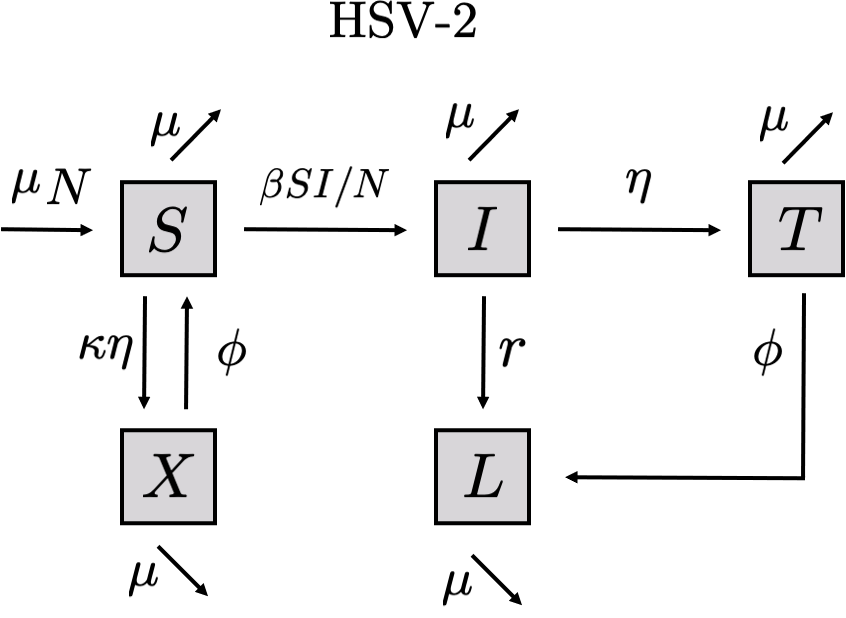
\includegraphics[width = 0.6\textwidth]{Flowcharts/hsv-2.png}
    \caption{Flowchart of HSV-2 disease model}
    \label{fig:hsv2_flow}
\end{figure}

The model considers susceptible individuals ($S$), individuals in early treatment ($X$), infected infectious individuals ($I$), infected individuals under treatment ($T$), and infected but not infectious individuals in a latent state ($L$). Susceptible individuals showing symptoms similar to HSV-2 infection can be sent to early treatment $X$ even if they are not HSV-2 infected, at rate $\kappa \eta$. Notice that also false positives may be sent to the $X$ class. After a treatment period, individuals in $X$ come back to $S$ at rate $\phi$.
Susceptible individuals get infected and progress to $I$ by contacting infectious individuals not in treatment. An infectious individual may go to a Latency state $L$ at rate $\gamma$, may go to treatment at rate $\eta$, or may die out at rate $\mu$.
Individuals under treatment progress to a dormant state $L$ at rate $\phi$ or dies out at rate $\mu$. Individuals in the latency state may develop symptoms and go to $I$ at rate $r$ or die out at rate $\mu$.

$$
\begin{aligned}
\frac{d S}{d t} &=\mu N+\phi X-\frac{\beta S I}{N}-(\mu+\kappa \eta) S \\
\frac{d X}{d t} &=\kappa \eta S-(\phi+\mu) X \\
\frac{d I}{d t} &=\frac{\beta S I}{N}+r L-(\eta+\gamma+\mu) I \\
\frac{d T}{d t} &=\eta I-\left(\phi+\mu\right) T \\
\frac{d L}{d t} &=\gamma I+\phi T-(r+\mu) L
\end{aligned}
$$


\subsection*{Model Analysis}

Using the Next Generation Matrix (NGM) to derive the control reproductive number and the basic reproduction number $\mathcal{R}_0$, we define the infectious compartments $\{I,T,L\}$. Since the total population is at steady state $\dot{N}=0$, the Disease-Free Equilibrium (DFE) in the presence of treatment is given by
$$
\left(\frac{N(\mu+\phi)}{\kappa \eta+\mu+\phi}, \frac{N\kappa \eta}{\kappa \eta+\mu+\phi}, 0,0,0\right).
$$
\noindent We define
$\mathcal{F}=\left[\begin{array}{c}\frac{\beta S I}{N} \\ 0 \\ 0\end{array}\right] \quad$ and $\quad \mathcal{V}=\left[\begin{array}{c}(\eta+\gamma+\mu) I-r L \\ (\phi+\mu) T-\eta I \\ (\mu+r) L-\gamma I-\phi T\end{array}\right]$.

The Jacobian matrices for $\mathcal{F}$ and $\mathcal{V}$ with respect to $I, T$ and $L$ evaluated at the DFE are respectively the following:

\noindent $F=\left[\begin{array}{lll}\beta & 0 & 0 \\ 0 & 0 & 0 \\ 0 & 0 & 0\end{array}\right]$
and $V=\left[\begin{array}{ccc}\gamma+\eta+\mu & 0 & -r \\ -\eta & \phi+\mu & 0 \\ -\gamma & -\phi & \mu+r\end{array}\right]$.
%
The spectral radius of the NGM, $FV^{-1}$ is then
\begin{equation}
\mathcal{R}_C=\frac{\frac{\beta}{\mu+\eta+\gamma} \cdot \frac{\mu+\phi}{\eta \kappa+\mu+\phi}}{1-\left(\frac{\gamma}{\eta+\mu+\gamma} \cdot \frac{r}{\mu+r}+\frac{\phi}{\mu+\phi} \cdot \frac{\eta}{\eta+\mu+\gamma} \cdot \frac{r}{\mu+r}\right)}
\end{equation}
Notice that $\mathcal{R}_C$ corresponds to the control reproductive number. The basic reproductive number is obtained by setting the control parameters $\phi,\eta$ to zero. Therefore
\begin{equation} \label{eq:hsv2brn}
\mathcal{R}_0=\frac{\frac{\beta}{\mu+\gamma}}{1-\frac{\gamma}{\mu+\gamma} \cdot \frac{r}{\mu+r}}.
\end{equation}

%\textcolor{purple}{smriti: A little confused here as to how the control reproductive number has been deduced to be as in the equation. (I apologise as I don't have enough background in this area to connect the dots, but maybe a little explanation like in the previous section would be helpful for a person with little background on this to follow ?)}

\subsection*{Model remarks}
In the proposed model, infected individuals never recovers from the disease. Infectious individuals ($I$), may progress to a treatment state ($T$), and then progress to a latent state ($L$), from which it is possible to come back to the infectious state. Therefore, a single individual may be in the infectious compartment $I$ many times during his/her lifespan, producing secondary infections during each visit to the $I$ stage.
%
The basic reproductive number takes into account that 
\begin{equation} \label{eq:hsv2brnsrs}
\mathcal{R}_0=\frac{\frac{\beta}{\mu+\gamma}}{1-\frac{\gamma}{\mu+\gamma} \cdot \frac{r}{\mu+r}}=\sum_{n=0}^{\infty}\left(\frac{\beta}{\mu+\gamma}\right)\left(\frac{\gamma}{\mu+\gamma} \cdot \frac{r}{\mu+r}\right)^{n}.
\end{equation}

%\section{Influenza-like Illnesses (ILI)}

%=-=-=-=-=-=-=-=-=-=-=-=-=-=-=-=-=-=-=-=-=

\chapter{Airborne diseases}
\label{chapt:airborne}

\section{COVID-19}
Grenfell's SIRS model \cite{baker2020susceptible}.
\subsection*{Introduction}
\begin{figure}[H]
    \centering
    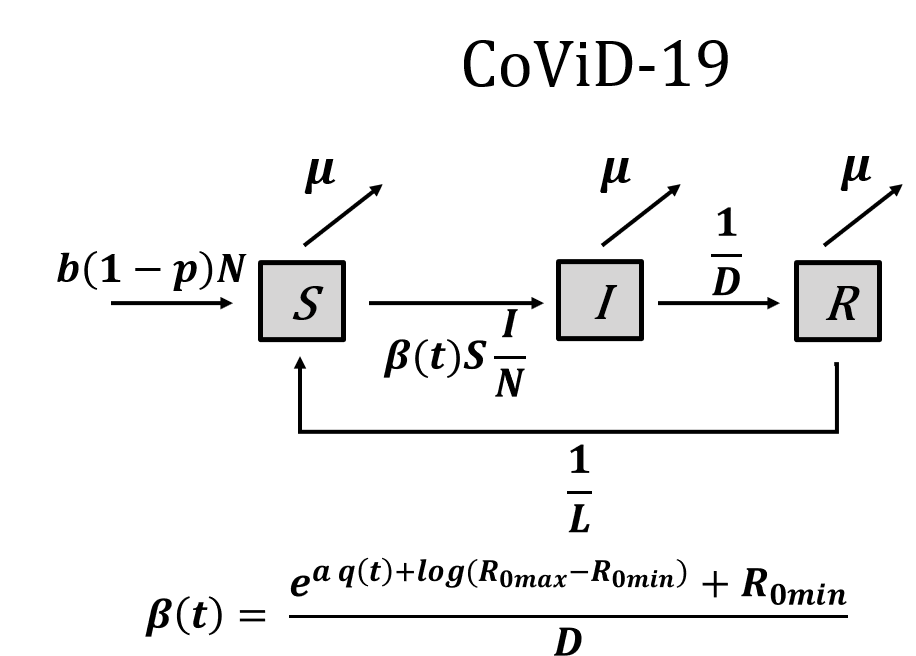
\includegraphics[width = 0.6\textwidth]{Flowcharts/covid.png}
    \caption{Flowchart of COVID-19 disease model}
    \label{fig:covid19_flow}
\end{figure}


\section{COVID-19 in the Mexican context}
\subsection{Introduction}
\subsection{Model}
The model in \cite{santamaria2020possible} study SARS-CoV-2 transmission in the Mexican context.
\begin{align}
\frac{\mathrm{d} S}{\mathrm{~d} t}&=\mu S-\left(k_{v}+k_{e} U+k_{i} I\right) S \\
\frac{\mathrm{d} U}{\mathrm{~d} t}&=\left(k_{v}+k_{e} U+k_{i} I\right) S-\alpha U \\
\frac{\mathrm{d} I}{\mathrm{~d} t}&=\alpha U-(\gamma r+\delta d+\epsilon a) I \\
\frac{\mathrm{d} A}{\mathrm{~d} t}&=\epsilon a I-[\delta p+\gamma(1-p)] A \\
\frac{\mathrm{d} R}{\mathrm{~d} t}&=\gamma r I+\gamma(1-p) A \\
\frac{\mathrm{d} D}{\mathrm{~d} t}&=\delta d I+\delta p A
\end{align}

\section{Tuberculosis}
\subsection*{Introduction}
Tuberculosis (TB) is a bacterial disease caused  by {\it Mycobacterium tuberculosis} with at least one-third of the world human population as its reservoir. %\textcolor{purple}{smriti: A citation might be required here?} 
TB remains the world’s deadliest infectious killer. 1.4 million people died from TB in 2019. %\cite{} 
%\textcolor{red}{This might not be true as of 2020 since the paper was from 20 years ago.}

Following primary tuberculosis (TB)  infection, only  approximately  10\% of  individuals develop active TB. Most people are assumed to mount an effective immune response to the initial infection that limits proliferation of the bacilli and leads to long-lasting partial immunity both to further infection and to reactivation of latent bacilli remaining from the original infection. Infected individuals may develop active TB as a consequence of exogenous reinfection, i.e.,  acquiring  a  new  infection  from  another  infectious  individual.

\subsection*{Mathematical Model}
The model proposed in \cite{feng2000model} stratifies the population under study in Susceptible ($S$), Exposed ($E$), Infected ($I$) and individuals under treatment ($T$).
Due to the worldwide endemic situation of TB, the model incorporates demography processes by assuming a constant recruitment of susceptible individuals ($\Lambda$) and average lifespan $\frac{1}{\mu}$. 

\begin{figure}
    \centering
    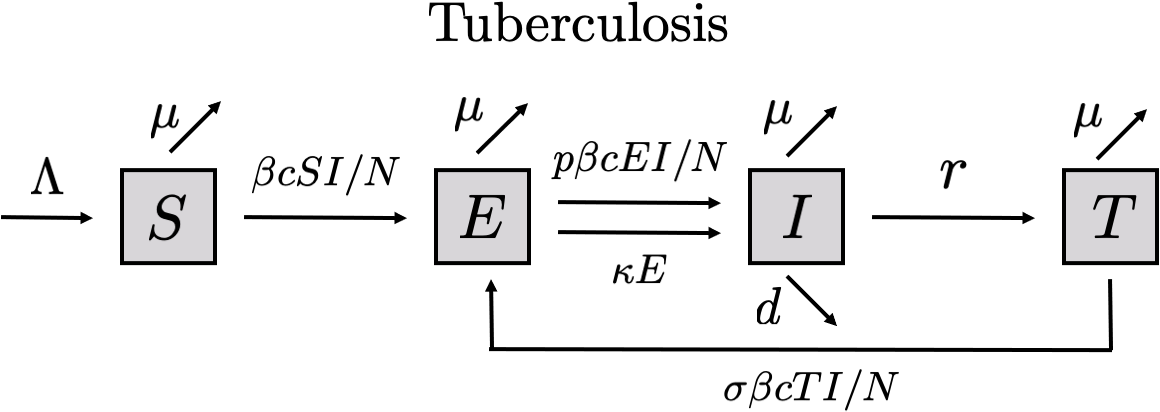
\includegraphics[width = 0.6\textwidth]{Flowcharts/tuberculosis.png}
    \caption{Flowchart of Tuberculosis disease model}
    \label{fig:tuberculosis_flow}
\end{figure}
Susceptible individuals become exposed by direct contacts with infected people at rate $\beta c S\frac{I}{N}$. Exposed individuals are assumed to become infectious by contacts with infected individuals at rate $p \beta c \frac{I}{N}$ or, by endogenous progression at rate $\kappa$, otherwise exposed individuals die out at rate $\mu$. Infectious individuals die out at rate $\mu$, receive treatment at rate $r$ or die out at rate $d$. Finally, individuals under treatment either become infectious again by contact with infected individuals at rate $\sigma \beta c \frac{I}{N}$ or die out at rate $\mu$.
$p$ represents the level of  reinfection, $c$ is the per-capita contact rate, and  $\leq\sigma\leq 1$ stands for a reduced infectiousness.
%
\begin{equation} \label{eq:TB_model}
\begin{array}{l}
\frac{d}{d t} S=\Lambda-\beta c S \frac{I}{N}-\mu S \\
\frac{d}{d t} E=\beta c S \frac{I}{N}-p \beta c E \frac{I}{N}-(\mu+k) E+\sigma \beta c T \frac{I}{N} \\
\frac{d}{d t} I=p \beta c E \frac{I}{N}+k E-(\mu+r+d) I \\
\frac{d}{d t} T=r I-\sigma \beta c T \frac{I}{N}-\mu T
\end{array}
\end{equation}
%
where $\mu=0.016 y^{-1}$, $d=0.1, p=0.4$, $\sigma=0.9, \Lambda=417(\Lambda / \mu=25000)$, $k=0.005$, $r=2$. The value of $\beta$ is calculated to be $7.465 y^{-1}$ for $R_0 = 0.87$ using the expression for the basic reproduction number shown in Equation \ref{eq:TB_basic}. Assuming $c = 1$, the system will show endemic equilibrium even for $R_0<1$ for the values of $p>0.3133$. Refer to Feng et. al. (2000) for the detailed analysis \cite{feng2000model}.

%\textcolor{red}{What is 25000 population of? What are the initial conditions? What region are these parameter values specific for? Original sources of the values required, since mathematical modeling papers use values from different places dated anytime in the past.}

\subsection*{Model Analysis}
In the absence of TB, the total population in model \eqref{eq:TB_model} is not constant, but it converges to a steady state
\begin{equation} \label{eq:TB_pop}
\frac{dN}{dt}=\frac{dS}{dt}+\frac{dE}{dt}+\frac{dI}{dt}+\frac{dT}{dt}=\Lambda-\mu N
\end{equation}
solving \eqref{eq:TB_pop}, we get that $N(t)\rightarrow \Lambda/\mu$. Using the next generation matrix, we can compute the basic reproductive number
\begin{equation}\label{eq:TB_basic}
\mathcal{R}_0= \left(\frac{\beta c}{\mu+r+d}\right)\left(\frac{k}{\mu+k}\right),
\end{equation}
the expression \eqref{eq:TB_basic} collects the secondary infections produced by the proportion of exposed individuals $\frac{k}{\mu+k}$, who become infectious and infects  at a rate $\beta c$ during their average infectious period $\frac{1}{\mu+r+d}$.

Notice that the basic reproductive number only captures the first time an individual is infected ($S\rightarrow E$) and not necessarily becomes infectious ($E\rightarrow I$). Moreover, $\mathcal{R}_0$ does not depend on $p$.

However, the endogenous infection ($\kappa E$) and treatment relapse ($\sigma \beta c T \frac{I}{N}$) are not captured in $\mathcal{R}_0$. This generates a {\it backward bifurcation}.
%
The key components of this type of dynamics are the processes associated to the relapse of individuals in latency state: endogenous progression $\kappa$, progression to treatment $r$ and, progression to latency $\sigma$.

\subsection*{Model Remarks}
The presented model studies the implication of exogenous and endogenous reinfection in the context of TB. The results suggest that these disease dynamics support an endemic equilibrium even when the classic metric $\mathcal{R}_0$ is less than one. This makes TB eradication more challenging because, while taking $\mathcal{R}_0<1$ is still necessary, it is not enough to guarantee a disease-free state. In this case, the system exhibits sensitivity to initial conditions if $\mathcal{R}_p<\mathcal{R}_0<1$, where $\mathcal{R}_p$ is a second threshold below which a disease-free state is guaranteed.

%\textcolor{red}{I was imagining the model remarks to be in terms of simulations and utility of COPASI codes of the diseases. Like ``TB is more prominent in one part of the world than other therefore introducing heterogeneity in transmission coefficient is important" or for HSV--2 ``women are x\% more likely to contract the disease than men, therefore considering sex-segregated model is needed for more accurate and realistic time course simulations".  }
%\textcolor{blue}{That's a good remark in terms of public health.}

% =-=-=-=-=-=-=-=-=-=-=-=-=-=-=-=-=-=-=-=-=

\section{Ebola virus disease}
\subsection*{Introduction}
Ebola virus disease (EVD) is transmitted to people from wild animals (such as fruit bats, porcupines and non-human primates) and then spreads in the human population through direct contact with the blood, secretions, organs or other bodily fluids of infected people, and with surfaces and materials (e.g. bedding, clothing) contaminated with these fluids.
%
The average EVD case fatality rate is around 50\%. Case fatality rates have varied from 25\% to 90\% in past outbreaks. There is no proven treatment for Ebola but simple interventions early on can significantly improve chances of survival.
%
The 2014–2016 outbreak in West Africa was the largest and most complex Ebola outbreak since the virus was first discovered in 1976. Around 30,000 infected cases and 11,000 deaths were reported during this outbreak.

\subsection*{Mathematical model}
In \cite{espinoza2018consequences}, the authors analyze the EVD dynamics in the absence of control measures. The mathematical model structures the population of interest by individuals' health states:
susceptible ($S$), exposed and possibly infectious individuals ($E$), symptomatic infectious and undiagnosed individuals ($I$) , disease-induced deaths ($D$) and recovered ($R$) individuals, $N=S+E+I+D+R$. 

\begin{figure}[H]
    \centering
    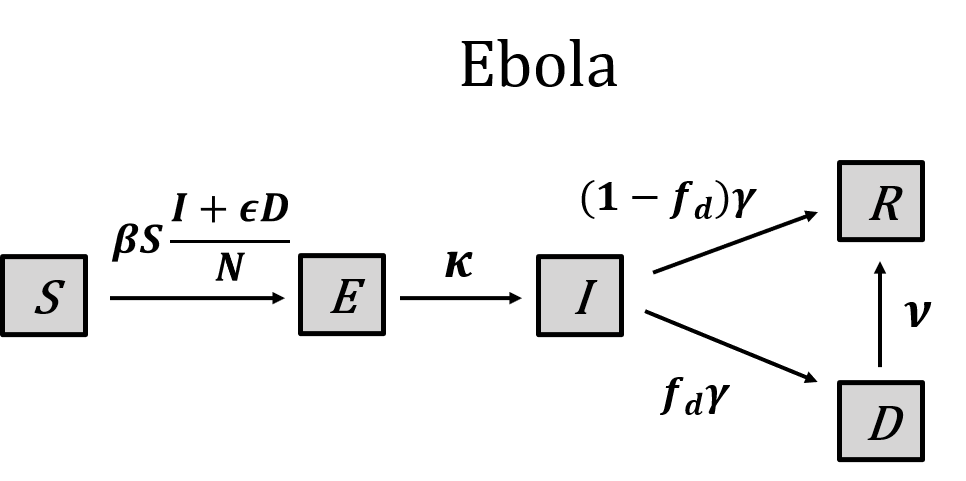
\includegraphics[width = 0.6\textwidth]{Flowcharts/ebola.png}
    \caption{Flowchart of Ebola disease model}
    \label{fig:ebola_flow}
\end{figure}

Susceptible individuals move to the infected compartment at rate $\beta\left(\frac{I+\varepsilon D}{N}\right)$ through ``effective'' contacts with either infected individuals $(I)$ or EVD-infected corpses $(D)$. Infected individuals spend on average $\frac{1}{\kappa}$ days on latency state, without being infectious. After the latency period, individuals become infectious $(I)$
on average during $\frac{1}{\gamma}$ days, after which, individuals either recover with probability $\left(1-f_{d}\right)$ or die with probability $f_{d}$. EVD-infected corpses $(D)$ subpopulation is assumed to increase at rate $f_{d} \gamma,$ and reduced through properly burial on average after $\frac{1}{v}$ days. EVD-infected corpses are assumed to be more infectious than infected individuals due to have the highest viral load, $\epsilon>1$.

\begin{equation} \label{eq:ebola_model}
\left\{\begin{array}{l}
\dot{S}=-\beta S\left(\frac{I+\varepsilon D}{N}\right) \\
\dot{E}=\beta S\left(\frac{I+\varepsilon D}{N}\right)-\kappa E \\
\dot{I}=\kappa E-\gamma I \\
\dot{D}=f_{\mathrm{d}} \gamma I-\nu D \\
\dot{R}=\left(1-f_{\mathrm{d}}\right) \gamma I+\nu D
\end{array}\right.
\end{equation}

%\textcolor{red}{$\kappa E$ flows out of E but only $(1-q)\kappa E$ goes into I. What happens to the rest?}
%\textcolor{blue}{That was a typo. Thanks}
%
\begin{figure}[H]
    \centering
    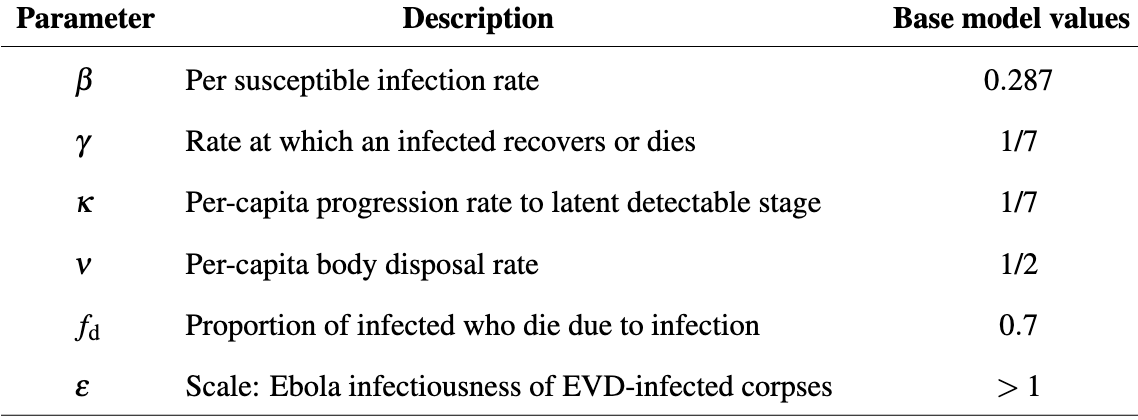
\includegraphics[scale=0.4]{ebola1}
    \caption{Parameters for Ebola model}
    \label{fig:ebola_params}
\end{figure}

\subsection*{Model analysis}
Model \eqref{eq:ebola_model} address a single EVD outbreak where the total population remain constant ($\dot{N}=\dot{S}+\dot{E}+\dot{I}+\dot{D}+\dot{R}$=0).
By using the next generation approach, with disease compartments $E, I, D$; the associated
basic reproductive number is
\begin{equation} \label{eq:brn_ebola}
\mathscr{R}_{0}=\beta\left(\frac{1}{\gamma}+\frac{\varepsilon f_{d}}{v}\right).
\end{equation}
The basic reproductive number of system \eqref{eq:ebola_model} captures the average number of secondary
infections produced by a typical infectious individual during their infectious period $\left(\frac{\beta}{\gamma}\right)$,
and the secondary cases generated by a single EVD-infected corpse, during its disposal
period $\left(\frac{\varepsilon \beta f_{d}}{v}\right),$ in a totally susceptible population.

%\subsection*{Simulations}
%\textcolor{red}{Units for parameters and references missing. What region are the included parameter values for? What are the initial conditions? Can you please share a screenshot of the figure that can be reproduced in this section?}

\subsection*{Model remarks}
The 2014 West African Ebola outbreak was a very challenging epidemic in great part due to the limitation of local public health infrastructure.
In order to address these challenges, the model \eqref{eq:ebola_model} incorporates two transmission routes: via infected individuals and via infected corpses. The model suggest that, while the main route of infection are the infected individuals, fast removal of infected corpses have a high impact on reducing $\mathcal{R}_0<1$ and thus in controlling an EVD outbreak.
Since births and deaths are not modeled here, users should run the time course for short time periods for more realistic results. The model can be extended to include control measures.
% =-=-=-=-=-=-=-=-=-=-=-=-=-=-=


\section{Measles}
\subsection*{Introduction}

\subsection*{Mathematical model}
In \cite{tessa2006mathematical}, the author considered a population composed by Susceptible individuals $S(t)$, Exposed individuals, but not yet infectious $E(t)$, Infectious individuals $I(t)$, and Recovered or removed artificially trough vaccination and permanently immune individuals $R(t)$.
%
The previously described disease dynamics are represented in the Figure \ref{fig:measles_flow}
\begin{figure}[H]
    \centering
    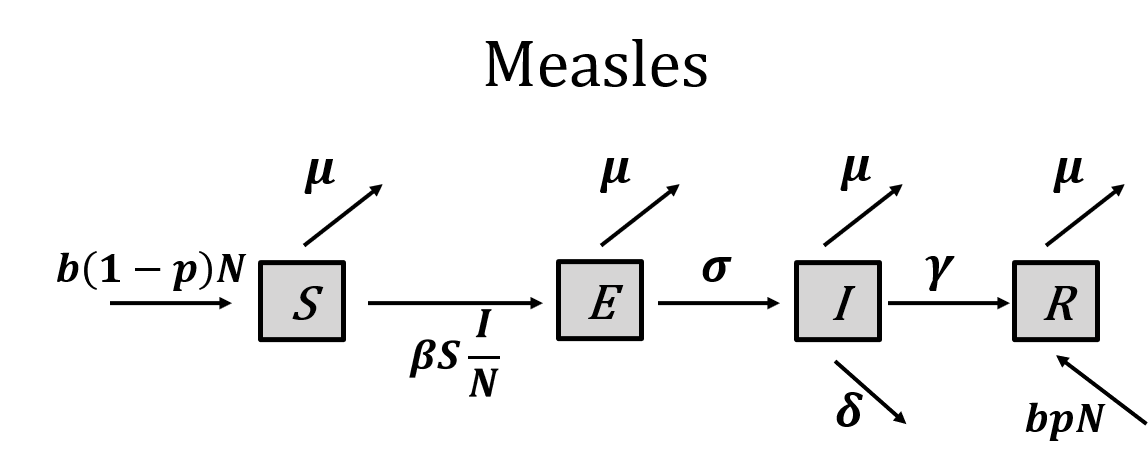
\includegraphics[width = 0.6\textwidth]{Flowcharts/measles.png}
    \caption{Flowchart of Measles disease model}
    \label{fig:measles_flow}
\end{figure}
%
and formalized by the set of ODE's \eqref{eq:measles}
\begin{equation}
\label{eq:measles}
\begin{aligned}
\frac{d S}{d t} &=b(1-p) N-\frac{\beta S I}{N}-\mu S \\
\frac{d E}{d t} &=\frac{\beta S I}{N}-(\sigma+\mu) E \\
\frac{d I}{d t} &=\sigma E-(\gamma+\mu+\delta) I \\
\frac{d R}{d t} &=b p N+\gamma I-\mu R
\end{aligned}
\end{equation}

\subsection*{Model analysis}
\subsection*{Model remarks}

% =-=-=-=-=-=-=-=-=-=-=-=-=-=-=-=

\section{Influenza}
\subsection*{Introduction}
Imperfect control measures to mitigate disease transmission are known to be mechanisms that may induce backward bifurcation \cite{gumel2012causes}. For example, imperfect quarantine or vaccines granting partial immunity for significantly short term periods.
In this section we use the work in \cite{erdem2017mathematical} to show how imperfect quarantine is modeled and some of its basic implications.

\subsection*{Mathematical model}
Consider the following model for Influenza and quarantine where $S, I, Q$ and $R$ correspond to the number of susceptible, infected, quarantine and recovered individuals, with $S+I+Q+R=N$. In this model
%
\begin{equation}
\begin{split}
  \dot{S} &= \mu N-\beta S \frac{I}{N-Q}-\mu S,\\
  \dot{I} &= \beta S \frac{I}{N-Q}-(\theta+\gamma+\mu) I,\\
  \dot{Q} &= \theta I-(\alpha+\mu) Q,\\
  \dot{R} &= \gamma I+\alpha Q-\mu R. 
  \end{split}
\end{equation}
%
In this model, a policy of perfect quarantine is considered. This impact the incidence term in the form $\beta S I /(N-Q)$ where $\beta$ is the per-capita effective contact rate.
%
The model assumes constant recovery ($\gamma$) and quarantine ($\theta$) per-capita rates. $\mu$ is the per-capita birth and death rate, and $\alpha$ is the per-capita recovery rate for isolated/quarantined individuals.

The aforementioned model assumes quarantine is perfect, and quarantined individuals cannot produce secondary infections during their quarantine period. However, in reality this usually is not true and we may expect certain leaking rate so that some quarantined individuals may infect others in the population. The following model incorporates infections of individuals undergoing quarantine
%
\begin{equation}
\label{model:impq}
\begin{split}
\frac{\mathrm{d} S}{\mathrm{~d} t} &=\mu N-\beta S \frac{I}{N-\sigma Q}-\hat{\beta} S \frac{(1-\sigma) Q}{N-\sigma Q}-\mu S \\
\frac{\mathrm{d} I}{\mathrm{~d} t} &=\beta S \frac{I}{N-\sigma Q}+\hat{\beta} S \frac{(1-\sigma) Q}{N-\sigma Q}-(\theta+\gamma+\mu) I \\
\frac{\mathrm{d} Q}{\mathrm{~d} t} &=\theta I-(\alpha+\mu) Q \\
\frac{\mathrm{d} R}{\mathrm{~d} t} &=\gamma I+\alpha Q-\mu R
  \end{split}
\end{equation}
%
Model \eqref{model:impq} incorporates imperfect quarantine for $\sigma\in[0,1]$. $\sigma=0$ stands for the scenario of totally ineffective quarantine, while $\sigma=1$ represents a totally perfect quarantine. Therefore, the total number of successfully quarantined individuals is $\sigma Q$ and therefore the total number of individuals who are available to mix homogeneously is $(N-\sigma Q)$.
%
In model \eqref{model:impq} $\hat{\beta}$ represents the effective rate of contacts between susceptible and imperfectly quarantined individuals.
%
Then, the proportion of contacts made with an infected individual is $I /(N-\sigma Q)$, while the proportion of contacts made with an imperfectly quarantined one is $(1-\sigma) Q /(N-\sigma Q)$. 
%
Therefore, the new force of infection is given by
\begin{equation}
\lambda=\beta \frac{I}{N-\sigma Q}+\hat{\beta} \frac{(1-\sigma) Q}{N-\sigma Q}
\end{equation}
%
where the new incidences due to contacts with infected individuals are $\beta S I /(N-\sigma Q)$, and due to contacts of susceptible with imperfectly quarantined individuals $\hat{\beta}(1-\sigma) S Q /(N-\sigma Q)$.

\subsection*{Model analysis}

To analyze model \eqref{model:impq} we normalize the model by assuming $N=1$ and letting $\hat{\beta}=r\beta$
%
\begin{equation}
\label{model:norm-impq}
\begin{split}
\frac{\mathrm{d} \bar{S}}{\mathrm{~d} t} &= \mu-\beta \bar{S} \frac{[\bar{I}+r(1-\sigma) \bar{Q}]}{1-\sigma \bar{Q}}-\mu \bar{S} \\
\frac{\mathrm{d} \bar{I}}{\mathrm{~d} t}&=\beta \bar{S} \frac{[\bar{I}+r(1-\sigma) \bar{Q}]}{1-\sigma \bar{Q}}-(\theta+\gamma+\mu) \bar{I} \\
\frac{\mathrm{d} \bar{Q}}{\mathrm{~d} t}&=\theta \bar{I}-(\alpha+\mu) \bar{Q} \\
\frac{\mathrm{d} \bar{R}}{\mathrm{~d} t}&=\gamma \bar{I}+\alpha \bar{Q}-\mu \bar{R}
\end{split}
\end{equation}
%
where $\bar{X}=X/N$ represents the proportion for the population in the health state $X$, so that $\bar{S}+\bar{I}+\bar{Q}+\bar{R}=1$.

\subsubsection*{Stability of the DFE}
By setting derivatives of the model \eqref{model:norm-impq} equal to zero, we get the system has the DFE $E_0=(1,0,0,0)$ and an endemic equilibrium.

To explore stability of $E_0$ we linearize the model around $E_0$ that shows a Jacobian matrix with two eigenvalues $-\mu$ and the eigenvalues of the submatrix
\begin{equation}
J_{0}=\left(\begin{array}{cc}
\beta-(\theta+\gamma+\mu) & (1-\sigma) r \beta \\
\theta & -(\alpha+\mu)
\end{array}\right).
\end{equation}
Thus, local stability is given by the conditions
\begin{align}
\operatorname{trace}\left(J_{0}\right)&=\beta-(\alpha+\mu)-(\theta+\gamma+\mu)<0\\
\operatorname{det}\left(J_{0}\right)&=(\alpha+\mu)(\gamma+\mu+\theta)-\beta(\alpha+\mu)-(1-\sigma) r \beta \theta>0
\end{align}
%
Re-arranging $\operatorname{det}\left(J_{0}\right)$ we get that in order for $E_0$ to be stable the following condition should hold
\begin{equation}
1>\frac{\beta}{\gamma+\mu+\theta}\left[1+(1-\sigma) \frac{r \theta}{\alpha+\mu}\right]=\mathcal{R}_0.
\end{equation}
Therefore, $E_0$ is stable whenever $\mathcal{R}_0<1$, and unstable whenever $\mathcal{R}_0>1$.

Furthermore, it is possible to show the model undergoes a Hopf bifurcation in the parameter space $(\sigma,\mathcal{R}_0,\theta)$.

\subsection*{Model remarks}
The present model incorporates two key consequences of assuming quarantine or isolation control measures: $(i)$ the proportion of the population homogeneously mixing changes under the assumption of quarantine/isolation, $(ii)$ the imperfect implementation of quarantine/isolation that may generate secondary cases.

% =-=-=-=-=-=-=-=-=-=-=

\section{Diphtheria}

\subsection*{Introduction}
The work in \cite{ilahi2018effectiveness} studies the 2017 Diptheria outbreak in Indonesia, that affected 28 provinces

\subsection*{Mathematical Model}

\begin{align}
\dot{S}&=A-\frac{(m-c) S I}{N}-(c+\mu) S+\gamma R \\
\dot{E}&=\frac{(m-c) S I}{N}-(\delta+\mu) E \\
\dot{I}&=\delta E-(\beta+\mu) I \\
\dot{R}&=\beta I+c S-(\gamma+\mu) R
\end{align}

\subsection*{Model analysis}
\subsection*{Model remarks}

% =-=-=-=-=-=-=-=-=-=-=-=
%  Vector-borne diseases
% =-=-=-=-=-=-=-=-=-=-=-=

\chapter{Vector-borne diseases}
\label{chapt:vectorborne}
%Dengue, Chikungunya, Malaria...

\section{Zika}
\subsection*{Introduction}
 Zika virus disease is caused by the bite of an infected Aedes species mosquito (\textit{Ae. aegypti} and \textit{Ae. albopictus}). These mosquitoes bite during the day and night.
 %\textcolor{purple}{smriti: we may be missing a citation here?}
 %
 Zika virus can be transmitted through sexual intercourse, and it can be passed from a pregnant woman to her fetus. Infection during pregnancy can cause microcephaly and other congenital malformations, known as congenital Zika syndrome. An increased risk of neurologic complications is associated with Zika virus infection in adults and children, including Guillain-Barré syndrome, neuropathy and myelitis. There is no treatment available for Zika virus infection or its associated diseases.

\subsection*{Mathematical model}

\begin{figure}
    \centering
    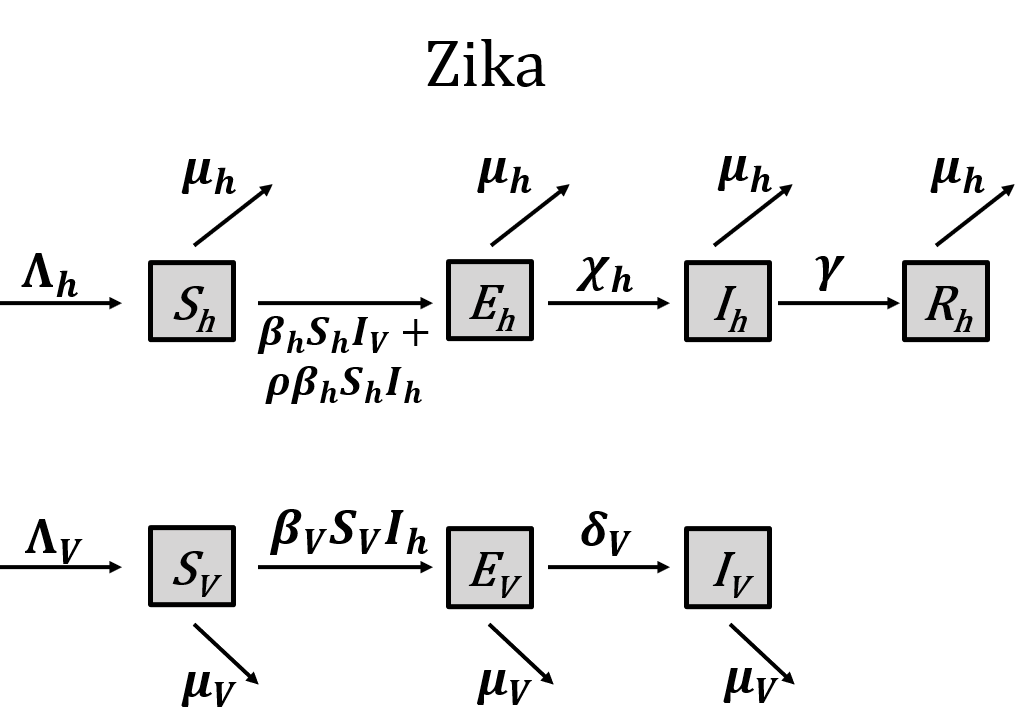
\includegraphics[width = 0.6\textwidth]{Flowcharts/zika.png}
    \caption{Flowchart of Zika disease model}
    \label{fig:zika_flow}
\end{figure}
In \cite{bonyah2017theoretical}, authors take into account the human to human infection as well as the vector (mosquito) to human transmission. The model subdivide the total human population, $N_{H}(t),$ into susceptible humans $S_{H}(t),$ exposed human $E_{H}(t),$ infected humans $I_{H}(t),$ and recovered humans $R_{H}(t),$ so that $N_{H}(t)=S_{H}+E_{H}+I_{H}+R_{H}$. The entire mosquito population, denoted by $N_{V}(t),$ is partitioned into susceptible vector $S_{V}(t),$ exposed vector $E_{V}(t)$ and infected mosquito $I_{V}(t)$ and hence $N_{V}=S_{V}+E_{V}+I_{V}$. The proposed model is

\begin{equation} \label{eq:zika_model}
\left\{\begin{array}{l}
\frac{d}{d t} S_{h}=\Lambda_{h}-\beta_{h} S_{h}\left(I_{V}+\rho I_{h}\right)-\mu_{h} S_{h} \\
\frac{d}{d t} E_{h}=\beta_{h} S_{h}\left(I_{V}+\rho I_{h}\right)-\left(\mu_{h}+\chi_{h}\right) E_{h} \\
\frac{d}{d t} I_{h}=\chi_{h} E_{h}-\left(\mu_{h}+\gamma+\eta\right) I_{h} \\
\frac{d}{d t} R_{h}=\gamma I_{h}-\mu_{h} R_{h} \\[2ex]
\frac{d}{d t} S_{V}=\Lambda_{V}-\beta_{V} S_{V} I_{h}-\mu_{V} S_{V} \\
\frac{d}{d t} E_{V}=\beta_{V} S_{V} I_{h}-\left(\mu_{V}+\delta_{V}\right) E_{V} \\
\frac{d}{d t} I_{V}=\delta_{V} E_{V}-\mu_{V} I_{V}
\end{array}\right.
\end{equation}

%\textcolor{red}{Where does the flow $\eta I_h$ go into? I think $N_h$ will also need a differential equation. The difference between $\gamma$ and $\eta$ unclear.}
%\textcolor{blue}{$\eta I_H$ represents disease-induced deaths while $\gamma I_H$ represents recoveries}


\subsection*{Mathematical analysis}
Notice the host population is not constant, so we start computing the host population steady state
\begin{equation} \label{eq:zika_host_pop}
    N'_h=S'_h+E'_h+I'_h+R'_h=\Lambda_h-\mu_h N_h-\eta_h I_h
\end{equation}
From equation\eqref{eq:zika_host_pop} we can obtain that in the absence of infection $N_h\rightarrow \frac{\Lambda_h}{\mu_h}$ and, in the presence of Zika infections
$$
N'_{h}+\mu_{h} N_{h} \leq \Lambda_{h}.
$$
The dynamics of vector population is described by $N'_{v}=\Lambda_{v}-\mu_{v} N_{v}$ which implies that $N'_{v}=\frac{\Lambda_v}{\mu_v}$.

The disease free equilibrium is given by $E_0=\{N_h,0,0,0,N_v,0,0\}$, and following the second-generation method
$$
F=\left(\begin{array}{cccc}
0 & \frac{\rho \beta_{h} \Lambda_{h}}{\mu_{h}} & 0 & \frac{\beta_{h} \Lambda_{h}}{\mu_{h}} \\
0 & 0 & 0 & 0 \\
0 & \frac{\beta_{v} \Lambda_{v}}{\mu_{V}} & 0 & 0 \\
0 & 0 & 0 & 0
\end{array}\right), V=\left(\begin{array}{cccc}
k_{1} & 0 & 0 & 0 \\
-\chi_{h} & k_{2} & 0 & 0 \\
0 & 0 & k_{3} & 0 \\
0 & 0 & -\delta_{V} & \mu_{V}
\end{array}\right)
$$
where $k_{1}=\mu_{h}+\chi_{h}, k_{2}=\left(\mu_{h}+\gamma+\eta\right)$ and $k_{3}=\left(\mu_{V}+\delta_{V}\right)$. The basic reproductive number of model \eqref{eq:zika_model} is  then the spectral radius of the matrix $FV^{-1}$
$$\mathcal{R}_{0}=\frac{\rho \beta_{h} \Lambda_{h} \chi_{h}}{2 \mu_{h} k_{1} k_{2}}+\sqrt{\frac{\rho^{2} \beta_{h}^{2} \Lambda_{h}^{2} \chi_{h}^{2}}{4 \mu_{h}^{2} k_{1}^{2} k_{2}^{2}}+\frac{\beta_{h} \Lambda_{h} \chi_{h} \beta_{V} \delta_{V} \Lambda_{V}}{\mu_{h} \mu_{V}^{2} k_{1} k_{2} k_{3}}}.$$

{\it Further analysis can be done on the endemic equilibria and the backward bifurcation.}

\subsection*{Simulations}
%\textcolor{red}{Some of the parameters don't have the units states in the table. Sources of the parameter values? Region for which these values hold true? Initial conditions?}

\begin{figure}[H]
    \centering
    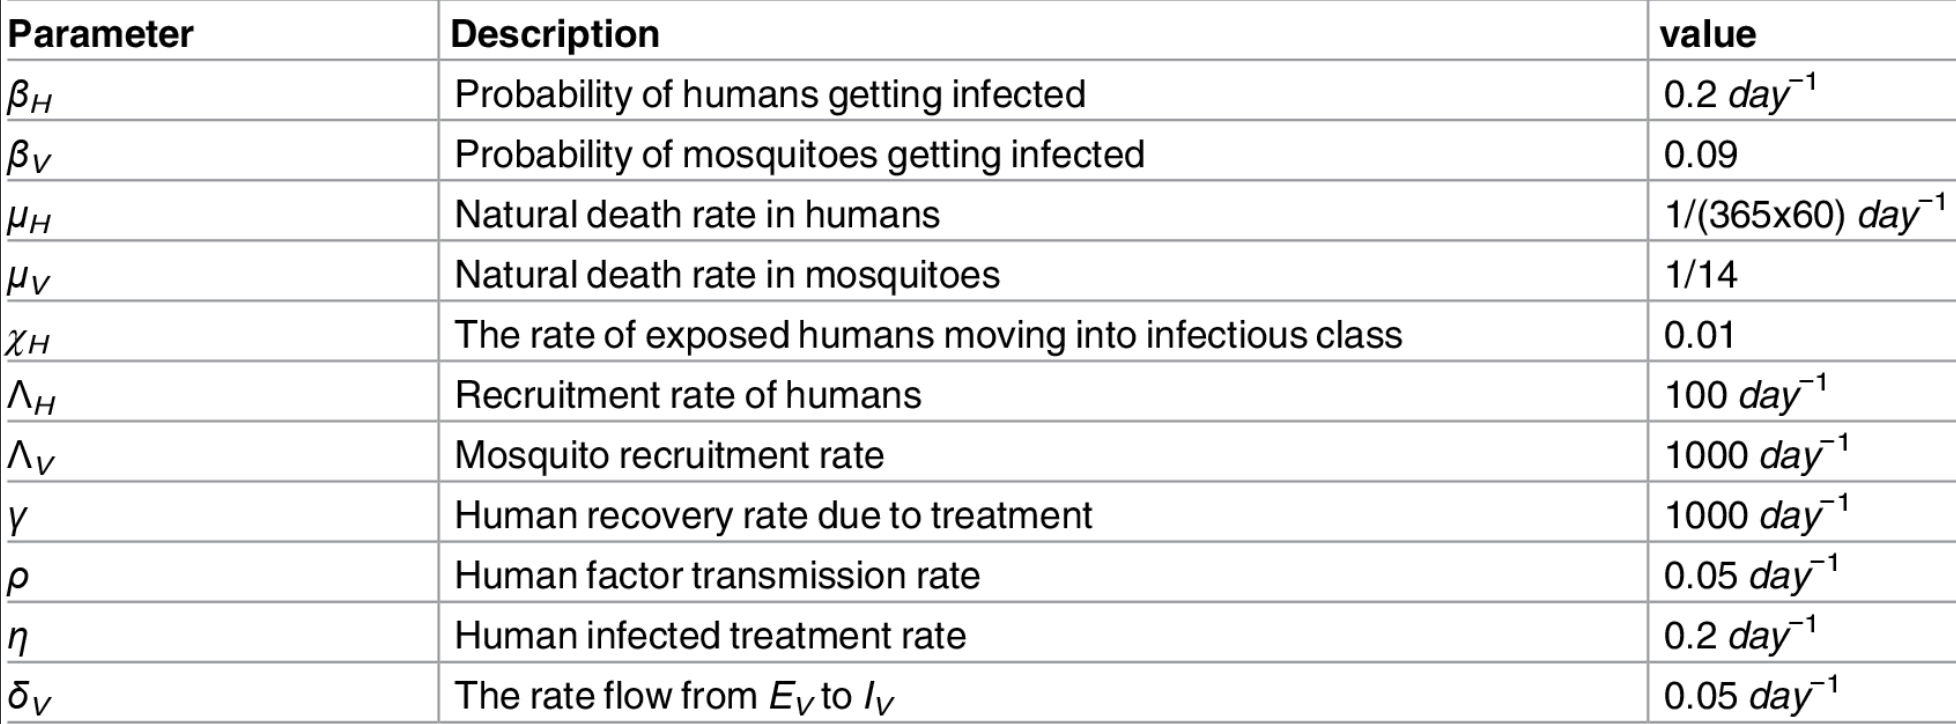
\includegraphics[scale=0.25]{zika1}
    \caption{Parameters for Zika model}
    \label{fig:zika_params}
\end{figure}

%\textcolor{purple}{smriti:confused here as to if the values in the table  calculated by the research team or are the parameters supposed to hold these values based on state of the art citations?}
%\textcolor{blue}{The parameter values for all models are the ones in the cited papers.}

Note: Initial condition $I_0$ different in reported best fit and in the plot in the paper \cite{bonyah2017theoretical}.
Estimated $\mu = 0.000457$; Figure 5 uses $\mu = 0.003199$.
%http://tabnet.datasus.gov.br/cgi/tabcgi.exe?sinannet/cnv/zikabr.def 

% =-=-=-=-=-=-=-=-=-=

\section{Malaria}

Malaria is a life-threatening disease transmitted back and forth between by vectors and hosts.
It is caused by parasites transmitted to people through the bites of infected female Anopheles mosquitoes.

\subsection*{Mathematical model}

Under the assumption that there are no hosts or vectors disease induced deaths, the hosts and mosquitoes populations remain constant, $N_h$ and $N_v$ respectively.
%
\begin{figure}[H]
    \centering
    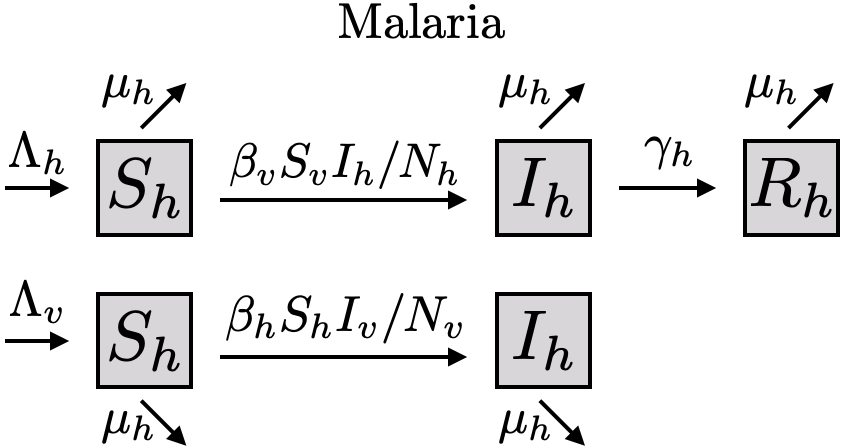
\includegraphics[width = 0.5\textwidth]{Flowcharts/malaria.png}
    \caption{Flowchart of Malaria disease model}
    \label{fig:malaria_flow}
\end{figure}

Following \cite{brauer2019mathematical}, a vector borne disease model for Malaria considers the interaction between the host population and mosquitoes population. Moreover, given that infected mosquitoes remain infected for life and do not recover, the proposed model assumes an SIR-like structure for both populations, but where mosquitoes never recover
%
\begin{align} 
\label{eq:malaria_model}
\nonumber S_{h}^{\prime}&=\Lambda_{h}-\beta_h S_{h} \frac{I_{v}}{N_{v}}-\mu_{h} S_{h} \\
 I_{h}^{\prime}&=\beta_h S_{h} \frac{I_{v}}{N_{v}}-\left(\mu_{h}+\gamma_{h}\right) I_{h} \\
\nonumber S_{v}^{\prime}&=\Lambda_{v}-\beta_v S_{v} \frac{I_{h}}{N_{h}}-\mu_{v} S_{v} \\
\nonumber I_{v}^{\prime}&=\beta_v S_{v} \frac{I_{h}}{N_{h}}-\mu_{v} I_{v}
\end{align}
%

\subsection*{Model analysis}
Notice that in model \eqref{eq:malaria_model} the host population is not constant since
\begin{equation} \label{eq:malaria_host_pop}
   N'_h=S'_h+I'_h=\Lambda_h-\mu_h N'_h.
\end{equation}
In order to explicitly find the equilibrium of the host population, we solve equation \eqref{eq:malaria_host_pop}. The total host population is then given by $$N(t)=N(0)e^{-\mu t}+\frac{\Lambda_h}{\mu_h}.$$ By the theory of asymptotic systems, we can analyze system's \eqref{eq:malaria_model} qualitative behavior by assuming the population involved already reached its steady state. Since $N(t)\rightarrow \frac{\Lambda_h}{\mu_h}$, we get that model's \eqref{eq:malaria_model} has a disease-free equilibrium $(N_h,0,N_v,0)$, where $N_h=\frac{\Lambda_h}{\mu_h}$ and $N_v=\frac{\Lambda_v}{\mu_v}$. 

Demographic processes in the hosts and mosquitoes population allow for an endemic equilibrium under the following conditions
\begin{align}
\nonumber \beta_{h} S_{h} I_{v} &=\left(\gamma_{h}+\mu_{h}\right) I_{h} N_{v} \\
\nonumber \beta_{v} S_{v} I_{h} &=\mu_{v} I_{v}N_h \\
 \Lambda_{h} &=S_{h}\left(\mu_{h}+\beta_{h} \frac{I_{v}}{N_{v}}\right) N_{v} \\
\nonumber \Lambda_{v} &=S_{v}\left(\mu_{v}+\beta_{v} \frac{I_{h}}{N_{h}}\right)N_{h}
\end{align}
%
By applying the second generation matrix to compute model's \eqref{eq:malaria_model} basic reproductive number, we get
$$
F=\left[\begin{array}{cc}
0 & \beta_{h} \frac{N_{h}}{N_{v}} \\
\beta_{v} \frac{N_{v}}{N_{h}} & 0
\end{array}\right], \quad V=\left[\begin{array}{cc}
\gamma_{h}+\mu_{h} & 0 \\
0 & \mu_{v}
\end{array}\right]
$$
where the second generation matrix is
$$
F V^{-1}=\left[\begin{array}{cc}
0 & \frac{\beta_{h} \frac{N_{h}}{N_{v}}}{\mu_{v}} \\
\frac{\beta_{v} \frac{N_{v}}{N_{h}}}{\gamma_{h}+\mu_{h}} & 0
\end{array}\right]
$$
and the basic reproductive number
\begin{equation} \label{eq:malaria_brn}
\mathscr{R}_{0}=\sqrt{\frac{\beta_{h} \beta_{v}}{\mu_{v}\left(\gamma_{h}+\mu_{h}\right)}}.
\end{equation}

\subsection*{Model remarks}
Notice that following this approach, expression \eqref{eq:malaria_brn} envision human-human transmission as a two step process: human-vector and vector-human transmission. However, it may be more appropriate to consider both steps as a single process producing the next generation of infected hosts. Under the former assumption, expression \eqref{eq:malaria_brn} becomes
\begin{equation}
\mathscr{R}_{0}=\frac{\beta_{h} \beta_{v}}{\mu_{v}\left(\gamma_{h}+\mu_{h}\right)}
\end{equation}
%
Notice that in both cases, the epidemic threshold for disease eradication or disease persistence is the same, $\mathcal{R}_0=1$.

%Discuss about $\beta$ meaning change if we consider $\frac{I_v}{N_v}$ or $\frac{I_v}{N_h}$.

\section{Dengue model}

\subsection*{Introduction}
Dengue is caused by a virus of the Flaviviridae family, mainly transmitted by the Aedes aegypti mosquito as the primary vector.
%
There are four types of the virus causing dengue fever (DENV-1, DENV-2, DENV-3 and DENV-4).
%
While the number of dengue cases reported to WHO increased over 8 fold over the last two decades, current estimates indicate that 390 million dengue virus infections per year (95\% credible interval 284–528 million), of which 96 million (67–136 million) manifest clinically (with any severity of disease). Where reported deaths between the year 2000 and 2015 increased from 960 to 4032, \cite{world2014dengue}.

\subsection*{Mathematical model}
By following the model formulation in \cite{brauer2019mathematical}, the proposed model assumes a recruitment rate proportional to the population size for the host and vector populations. Moreover, the vector population's recruitment rate is assumed to be composed by newborn susceptible mosquitoes ($\mu_v(N_v-qI_v)$), and newborn infected mosquitoes ($q\mu_v I_v$).
%
\begin{align}
\label{eq:denguemodel}
\nonumber S_{h}^{\prime} &=\mu_{h} N_{h}-\beta_{h} S_{h}\frac{I_{v}}{N_{v}}-\mu_{h} S_{h}, \\
\nonumber E_{h}^{\prime} &=\beta_{h} S_{h} \frac{I_{v}}{N_{v}}-\left(\eta_{h}+\mu_{h}\right) E_{h}, \\
\nonumber I_{h}^{\prime} &=\eta_{h} E_{h}-\left(\gamma+\mu_{h}\right) I_{h},\\
R_h &= \gamma I_h,\\
\nonumber S_{v}^{\prime} &=\mu_{v}\left(N_{v}-qI_{v}\right)-\beta_{v} S_{v} \frac{I_{h}}{N_{h}}-\mu_{v} S_{v}, \\
\nonumber E_{v}^{\prime} &=\beta_{v} S_{v} \frac{I_{h}}{N_{h}}-\left(\eta_{v}+\mu_{v}\right) E_{v}, \\
\nonumber I_{v}^{\prime} &=q \mu_{v} I_{v}+\eta_{v} E_{v}-\mu_{v} I_{v}.
\end{align}

\subsection*{Model analysis}
Following the second generation matrix with infectious compartments $\{E_h,I_h,E_v,I_v\}$, we get a basic reproductive number of the form
\begin{equation}
    \mathcal{R}_0=\beta_{h} \beta_{v} \frac{1}{\mu_{h}+\gamma} \frac{\eta_{v}}{\eta_{v}+\mu_{v}} \frac{\eta_{h}}{\eta_{h}+\mu_{h}} \frac{1}{\mu_{v}}+q\mu_v.
\end{equation}

\subsection*{Model remarks}
The model assumes a period of latency where neither hosts and vectors are infections, the dynamics of this model are similar to the SIR model where the latency period adds a delay in infections. Furthermore, the model assumes vertical transmission among the infected mosquitoes population (that is, infected mosquitoes produce infected newborns mosquitoes), which in turn impact the basic reproductive number and the disease eradication threshold.

\section{Leishmaniasis}
%
\subsection*{Introduction}

\subsection*{Mathematical model}
The modeling work by ELmojtaba et. al. \cite{elmojtaba2010mathematical}, assumes Leishmaniasis dynamics among three independent populations: human hosts ($N_H$), vectors ($N_V$)  and reservoirs ($N_R$).
%
Beyond the susceptible, infected and recovered health classes, the model assumes that humans after the treatment of visceral leishmaniasis may develop post kala-azar dermal leishmaniasis (PKDL).

The proposed model assumes two infection cycles: first, the infected reservoir population infect susceptible vectors, and susceptible reservoirs are infected by infected vectors; second, the infected vector population infect susceptible humans hosts, and infected human hosts infect susceptible mosquitoes.

\begin{figure}[H]
    \centering
    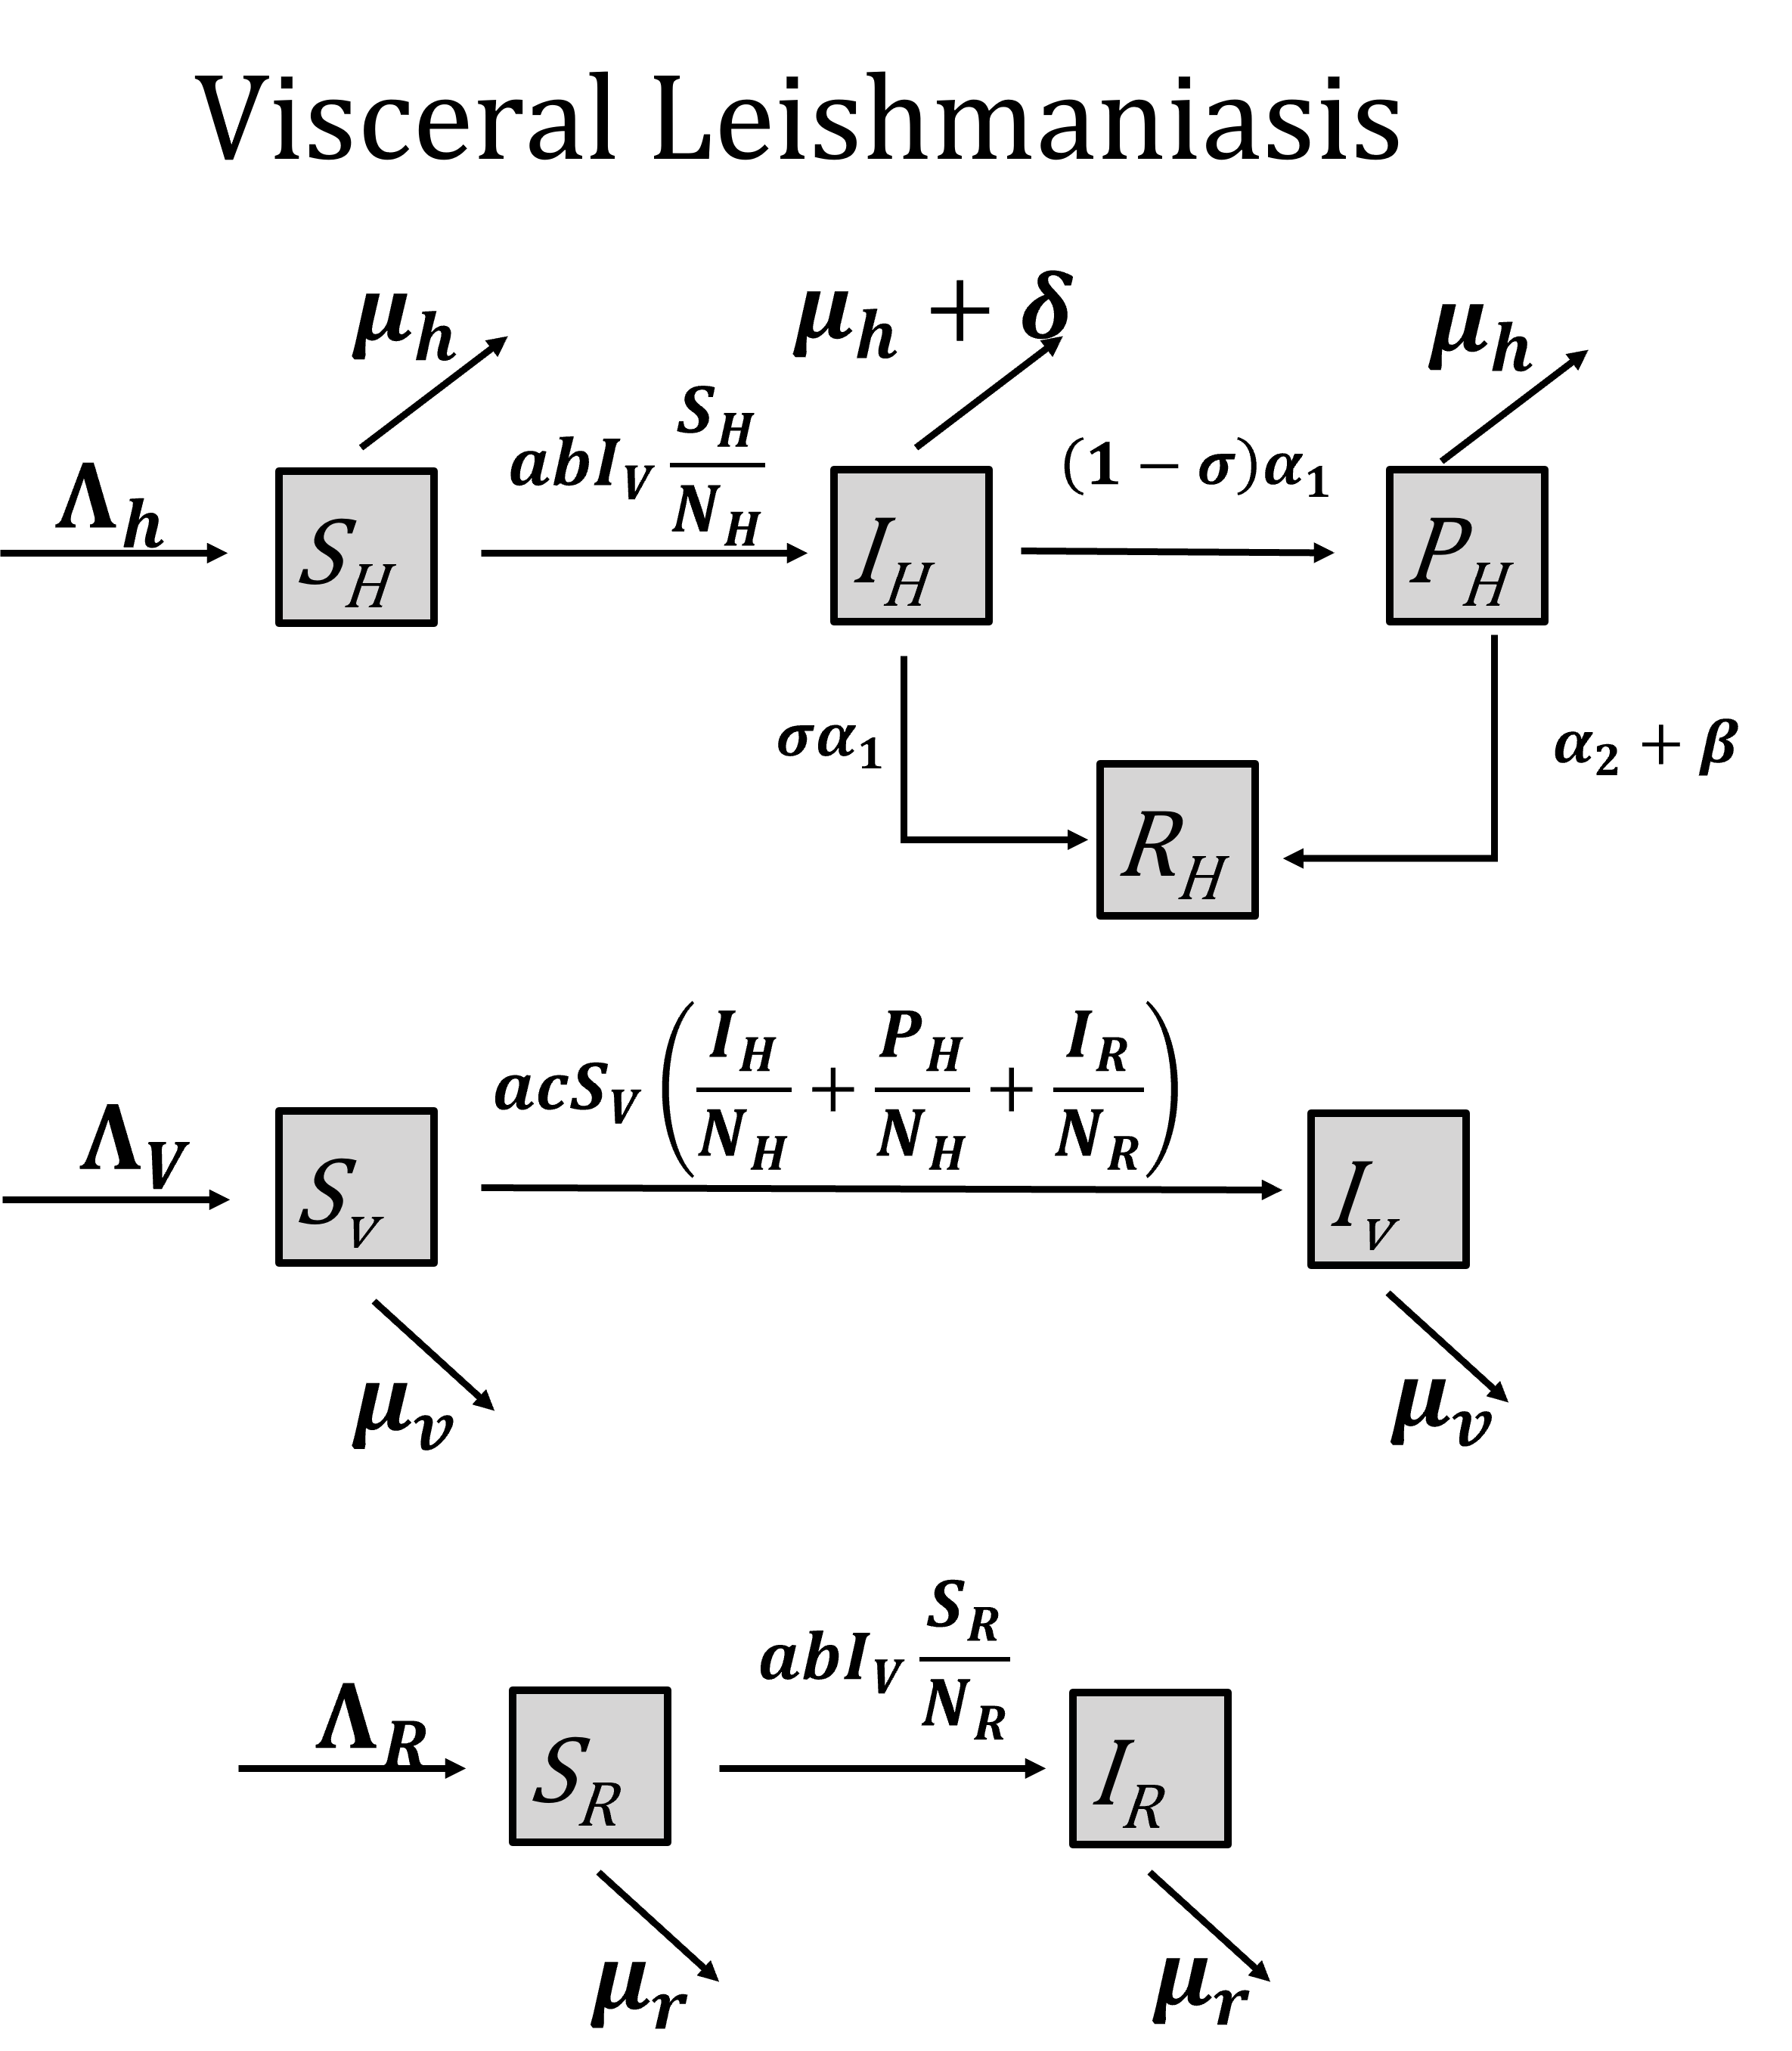
\includegraphics[width = 0.5\textwidth]{Flowcharts/visceralleishmaniasis.png}
    \caption{Flowchart of Visceral Leishmaniasis disease model}
    \label{fig:leishmaniasis_flow}
\end{figure}

\begin{equation}
\begin{split}
S_{H}^{\prime}&=\Lambda_{H}-a b I_{V} \frac{S_{H}}{N_{H}}-\mu_{h} S_{H} \\
I_{H}^{\prime}&=a b I_{V} \frac{S_{H}}{N_{H}}-\left(\alpha_{1}+\delta+\mu_{h}\right) I_{H} \\
P_{H}^{\prime}&=(1-\sigma) \alpha_{1} I_{H}-\left(\alpha_{2}+\beta+\mu_{h}\right) P_{H} \\
R_{H}^{\prime}&=\sigma \alpha_{1} I_{H}+\left(\alpha_{2}+\beta\right) P_{H}-\mu_{h} R_{H} \\
S_{R}^{\prime}&=\Lambda_{R}-a b I_{V} \frac{S_{R}}{N_{R}}+\mu_{r} S_{R} \\
I_{R}^{\prime}&=a b I_{V} \frac{S_{R}}{N_{R}}-\mu_{r} I_{R} \\
S_{V}^{\prime}&=\Lambda_{V}-a c S_{V} \frac{I_{H}}{N_{H}}-a c S_{V} \frac{P_{H}}{N_{H}}-a c S_{V} \frac{I_{R}}{N_{R}} S_{V}-\mu_{v} S_{V} \\
I_{V}^{\prime}&=a c S_{V} \frac{I_{H}}{N_{H}}+a c S_{V} \frac{P_{H}}{N_{H}}+a c S_{V} \frac{I_{R}}{N_{R}} S_{V}-\mu_{v} I_{V}
\end{split}
\end{equation}

\subsection*{Mathematical analysis}
The basic reproductive number of the proposed model is
\begin{equation}
\mathcal{R}_0=
\sqrt{\frac{a c\left[\mu_{r} a b m\left(\alpha_{2}+\beta+\mu_{h}+(1-\sigma) \alpha_{1}\right)+a b n\left(\alpha_{1}+\delta+\mu_{h}\right)\left(\alpha_{2}+\beta+\mu_{h}\right)\right]}{\mu_{r} \mu_{v}\left(\alpha_{1}+\delta+\mu_{h}\right)\left(\alpha_{2}+\beta+\mu_{h}\right)}}
\end{equation}

\subsection*{Model remarks}
The proposed model assumes a double infection cycle among three independent populations. In consequence, disease eradication is not guaranteed by treating the human host population, since the disease may persist for long periods among vectors and reservoirs.

\section{Yellow fever}

\subsection*{Introduction}

\subsection*{Mathematical model}
Based in the work by Zhao et. al. \cite{zhao2018modelling}.

\begin{equation}
\begin{split}
S_{h}^{\prime} &=-a b \frac{I_{u}}{N_{k}} S_{h}-v\left(t-t_{0}\right) \\
E_{h}^{\prime} &=a b \frac{I_{r}}{N_{h}} S_{h}-\sigma_{h} E_{h} \\
A_{h}^{\prime} &=(1-\delta) \sigma_{h} E_{h}-\gamma_{h} A_{h} \\
I_{h}^{\prime} &=\delta \sigma_{h} E_{h}-\gamma_{h} I_{h} \\
T_{h}^{\prime} &=\gamma_{h} I_{h}-\kappa_{h} T_{h} \\
R_{h}^{\prime} &=v\left(t-t_{0}\right)+\gamma_{h} A_{h}+(1-\theta) \kappa_{h} T_{h} \\
D_{h}^{\prime} &=\theta \kappa_{h} T_{h} \\[2ex]
S_{v}^{\prime} &=B_{v}(t)-a c \frac{\psi d_{h}+I_{h}}{N_{k}} S_{v}-\mu_{v} S_{v} \\
E_{v}^{\prime} &=a c \frac{\psi A_{k}+I_{j}}{N_{k}} S_{v}-\sigma_{v} E_{v}-\mu_{v} E_{v} \\
I_{v}^{\prime} &=\sigma_{v} E_{v}-\mu_{v} I_{v}
\end{split}
\end{equation}

\subsection*{Model analysis}
The basic reproductive number of the model is 
\begin{equation}
\mathcal{R}_{0}=\sqrt{[\psi \cdot(1-\delta)+\delta] \cdot \frac{a^{2} b c m}{\gamma_{h}} \cdot \frac{\sigma_{v}}{\mu_{v}\left(\sigma_{v}+\mu_{v}\right)}}
\end{equation}

\subsection*{Model remarks}

% =-=-=-=-=-=-=-=-=-=-=-=-=-=-=-=-=-=-=-=-=-=-=-=-=

\chapter{Generic Models}
\label{chapt:genmods}

\section{A two-strains model}

From the book by Martcheva \cite{martcheva2015introduction}. Consider an SIR model with  genetic variability of a non-fatal infectious pathogen. The population is divided into susceptible individuals $S$, individuals infected by strain one $I_{1}$, individuals infected by strain two $I_{2}$, and recovered individuals $R(t)$. Assume recovered individuals get permanent cross-immunity after being infected. In other words, after infected with a strain they can't being infected with the same or the other strain.
%
In addition, assume differential infectiousness on the strains $\beta_1$ and $\beta_2$ as well as variable serial periods $\alpha_1$ and $\alpha_2$.

The previously described model of disease progression is given by 
\begin{equation} \label{eqn:twostmod}
\begin{array}{l}
S^{\prime}=\Lambda-\beta_{1} \frac{S I_{1}}{N}-\beta_{2} \frac{S I_{2}}{N}-\mu S \\
I_{1}^{\prime}=\beta_{1} \frac{S I_{1}}{N}-\left(\mu+\alpha_{1}\right) I_{1} \\
I_{2}^{\prime}=\beta_{2} \frac{S I_{2}}{N}-\left(\mu+\alpha_{2}\right) I_{2} \\
R^{\prime}=\alpha_{1} I_{1}+\alpha_{2} I_{2}-\mu R
\end{array}
\end{equation}

Adding model's \ref{eqn:twostmod} equations, we get that the total population $N$ is described by $N'(t)=\Lambda-\mu N$.
%
Model \ref{eqn:twostmod} has three equilibria: a disease free-equilibrium given by $\mathcal{E}^*=\{\frac{\Lambda}{\mu},0,0,0\}$, and two endemic equilibria where each of the strains dominates.

Notice that the strain-specific reproduction number are given by $\mathcal{R}_k=\frac{\beta_k}{\mu+\alpha_k}$. Opposite to the single strain SIR model, the DFE $\mathcal{E}^*$ is stable if both reproduction numbers are less than one, and the DFE becomes unstable if at least one of the reproduction numbers is greater than one.

\subsection*{The strain-specific dominance}
By changing the model variables to proportions we get that $s=\frac{S}{N}$, $i_{k}=\frac{I_{k}}{N}$, and since at the steady state $\Lambda=\mu N$, we get that the equilibria are given by

\begin{equation} \label{eq:propmod}
\begin{array}{l}
0=\mu-\beta_{1} s i_{1}-\beta_{2} s i_{2}-\mu s \\
0=\beta_{1} s i_{1}-\left(\mu+\alpha_{1}\right) i_{1} \\
0=\beta_{2} s i_{2}-\left(\mu+\alpha_{2}\right) i_{2} \\
0=\alpha_{1} i_{1}+\alpha_{2} i_{2}-\mu r
\end{array}
\end{equation}

The strain specific dominance is given by the absence of infected individuals of the other strain. Assuming that strain 1 becomes dominant, we get $I_1\neq 0$ and $I_2=0$. Therefore, we get that $s=\frac{\mu+\alpha}{\beta_1}=\frac{1}{\mathcal{R}_1}$. Notice that $s$ is a proportion of the population, so that this holds whenever $\mathcal{R}_1>1$.

From \eqref{eq:propmod} we get 
\begin{equation}
\frac{\mu}{s}=\beta_{1} i_{1}+\mu
\end{equation}
and
\begin{equation}
\begin{aligned}
i_{1} &=\frac{\mu}{\left(\mu+\alpha_{1}\right) \mathscr{R}_{1}}=\frac{\mu}{\mu+\alpha_{1}}\left(1-\frac{1}{\mathscr{R}_{1}}\right) \\
r &=\frac{\alpha_{1}}{\mu} i_{1}=\frac{\alpha_{1}}{\mu+\alpha_{1}}\left(1-\frac{1}{\mathscr{R}_{1}}\right).
\end{aligned}
\end{equation}

Therefore the strain-one dominance equilibrium is given by
\begin{equation}
\mathscr{E}_{1}=\left(\frac{1}{\mathscr{R}_{1}} \frac{\Lambda}{\mu}, \frac{\mu}{\mu+\alpha_{1}}\left(1-\frac{1}{\mathscr{R}_{1}}\right) \frac{\Lambda}{\mu}, 0, \frac{\alpha_{1}}{\mu+\alpha_{1}}\left(1-\frac{1}{\mathscr{R}_{1}}\right) \frac{\Lambda}{\mu}\right)
\end{equation}

Similarly, the strain-two dominance equilibrium is given by
\begin{equation}
\mathscr{E}_{2}=\left(\frac{1}{\mathscr{R}_{2}} \frac{\Lambda}{\mu}, 0, \frac{\mu}{\mu+\alpha_{2}}\left(1-\frac{1}{\mathscr{R}_{2}}\right) \frac{\Lambda}{\mu}, \frac{\alpha_{2}}{\mu+\alpha_{2}}\left(1-\frac{1}{\mathscr{R}_{2}}\right) \frac{\Lambda}{\mu}\right)
\end{equation}

This model highlights the {\bf Competitive Exclusion Principle:} When $n$ strains compete in a population, the strain with the largest reproduction number outcompetes the other strains and drives them to extinction.

However, there are mechanisms that allow stable coexistence of multiple pathogens in an epidemic model, namely {\it mutation, coinfection, superinfection, } 

\section{A model with linear likelihood of infection}

From the book by Martcheva \cite{martcheva2015introduction}. Assume a constant population composed by Susceptible $S$, Infected $I$ and Recovered $R$ individuals. Assume also the transmission coefficient is linear in the number of infected individuals $1+\nu I$ where $\nu>1$, for instance, due to an increase in the number of contacts or an increased probability of infection.

\begin{align} \label{eq:nonc}
\nonumber S^{\prime}(t) &=\Lambda-\beta(1+v I) I S-\mu S\\
I^{\prime}(t) &=\beta(1+v I) I S-(\alpha+\mu) I\\
\nonumber R'(t)&=\alpha I-\mu R
\end{align}

%\subsection{Model analysis}
Adding model \eqref{eq:nonc} equations, we get that the total population $N$ is described by $N'(t)=S'(t)+I'(t)+R'(t)=\Lambda-\mu N$, which solution converges to the steady state $N^*=\frac{\Lambda}{\mu}$. Therefore the disease free equilibrum always exists and it is given by $\mathcal{E}^*=\{ \frac{\Lambda}{\mu},0,0 \}$.

The endemic equilibria is obtained by solving 
\begin{align} \label{eq:endnonc}
\Lambda-\beta(1+v I) I S-\mu S&=0\\
\beta(1+v I) I S-(\alpha+\mu) I&=0\\
\end{align}
from where we get that
\begin{equation} \label{eq:quadnonc}
(1+v I)\left[\frac{\Lambda}{\mu}-\frac{\mu+\alpha}{\mu} I\right]=\frac{\mu+\alpha}{\beta}.
\end{equation}
Notice that expression \eqref{eq:quadnonc} is a quadratic equation on $I$, which implies that under some scenarios there may exists one or two endemic equilibria.

Consider the left-hand size of the expression \eqref{eq:quadnonc}, and denote it by $f(I)$. The endemic equilibria of model \eqref{eq:nonc} are given by the intersections of the parabola $f(I)$ with the horizontal line $y=\frac{\mu+\alpha}{\beta}$.
Since $f(I)$ attains its maximum at \begin{equation}
I_{max}=\frac{1}{2 v}\left(\frac{\Lambda v}{\mu+\alpha}-1\right)
\end{equation}
then, there will be two endemic equilibria provided $I_{max}>y=\frac{\mu+\alpha}{\beta}$.

\section{A model with disease induced-deaths and treatment}
From: Mathematical epidemiology - F. Brauer

\begin{align}
S^{\prime} &=-\beta S[I+\delta T] \\ 
I^{\prime} &=\beta S[I+\delta T]-(\alpha+\gamma) I \\ 
T^{\prime} &=\gamma I-\eta T \\ N^{\prime} &=-(1-f) \alpha I-\left(1-f_{T}\right) \eta T 
\end{align}

with basic reproductive number

\begin{equation}
\mathcal{R}_{0}=\frac{\beta}{\alpha+\gamma}+\frac{\gamma}{\alpha+\gamma} \frac{\delta \beta}{\eta}
\end{equation}

\section{A model with closed solutions}
From: Mathematical epidemiology - F. Brauer

Assumes a disease sufficiently debilitates infected individuals so that only susceptible individuals can reproduce. Let us consider the model

\begin{equation}
\begin{array}{l}
S^{\prime}=r S-\beta S I-\mu S \\
I^{\prime}=\beta S I-(\mu+\alpha) I
\end{array}
\end{equation}

notice that, this model is analogous to the predator-prey Lotka-Volterra model of population dynamics.

The model has a disease free equlibrium $(0,0)$ and an endemic equilibrium $((\mu+\alpha) / \beta,(r-\mu) / \beta)$. Consider, 
\begin{equation}
\frac{d I}{d S}=\frac{I(\beta S-\mu-\alpha)}{S(r-\beta I)}
\end{equation}
by separation of variables
\begin{equation}
\int\left(\frac{r}{I}-\beta\right) d I=\int\left(\beta-\frac{\mu+\alpha}{S}\right) d S
\end{equation}
and integration gives
\begin{equation}
\beta(S+I)-r \log I-(\mu+\alpha) \log S=c
\end{equation}
where $c$ is a constant of integration. This implies that
\begin{equation}
V(S,I)=\beta(S+I)-r \log I-(\mu+\alpha) \log S
\end{equation}
is constant over each orbit $V(S,I)$ in the SI-plane. These orbits represent periodic solutions

% \subsection{A model with treatment}

% \begin{align}
    
% \end{align}

\chapter{The Final Epidemic Size}
\label{chapt:finsize}

Consider the Kermack-McKendrick model with Susceptible $S$, Infected $I$ and Recovered $R$ individuals, and assume recovered individuals are permanently immune. Where $\beta>0$ is the likelihood of infection and $\gamma>0$ is the recovery rate.
Assume that the population at $t=0$ is totally susceptible, so that $S(0)=N$, $I(0)=1$ and $R(0)=0$
\begin{align*}
\dot{S} &= -\beta S I\\
 \dot{I} &= \beta S I -\alpha I\\
 \dot{R} &= \alpha I
\end{align*}
%
Further description of the model can be found in the book {\it Mathematical Models in Population Biology and Epidemiology}, Section 9.2.

By adding the equations for susceptible and infected individuals we get
\begin{equation} \label{eq:fun1}
(S(t)+I(t))'=-\alpha I(t).
\end{equation}

Notice that $S(t)+I(t)$ is a positive ($S(t)$ and $I(t)$ are positive) and decreasing function (its derivative is negative), therefore the limit exists. Recall that the derivative of a positive decreasing function tends to zero, therefore $\alpha I(t)\rightarrow 0$, since $\alpha>0$ this implies $I(t)\rightarrow 0$. 
%
Hence
$$\lim_{t\rightarrow \infty} (S(t)+I(t))=\lim_{t\rightarrow \infty} S(t)+\lim_{t\rightarrow \infty}I(t)=S_{\infty},$$
%
integration on both sides of \eqref{eq:fun1}
\begin{align*}
(S(t)+I(t))' &= -\alpha I(t)\\
-\frac{1}{\alpha}(S(t)+I(t))' &= I(t)\\
-\frac{1}{\alpha}\int_0^{\infty} (S(t)+I(t))' dt &= \int_0^{\infty} I(t)dt
\end{align*}
%

\begin{align*}
\int_0^{\infty} I(t)dt=-\frac{1}{\alpha}\int_0^{\infty} (S(t)+I(t))' dt &= -\frac{1}{\alpha}(S_\infty+\underbrace{I_\infty}_{\rightarrow 0}-(\underbrace{S _0+I_0}_{N}))\\
&=\frac{1}{\alpha}(N-S_\infty)
\end{align*}
Now dividing  both sides of $\dot{S}$  by $S$
%
\begin{align*}
\frac{\dot{S}}{S}&=-\beta S I\\
\int_0^\infty \frac{\dot{S}(t)}{S(t)} dt&=-\beta \int_0^\infty  I(t)dt\\
\log(S)\Big|_{0}^\infty &= -\beta \int_0^\infty  I(t)dt\\
\log\left( \frac{S_0}{S_\infty}\right)  &= \beta \int_0^\infty  I(t)dt\\
&= \beta\frac{1}{\alpha}(N-S_\infty)\\
&= \frac{\beta N}{\alpha}\left( 1-\frac{S_\infty}{N}\right) 
\end{align*}
therefore
\begin{equation} \label{eq:fins1}
    \log\left( \frac{S_0}{S_\infty}\right)  = \mathcal{R}_0\left( 1-\frac{S_\infty}{N}\right).
\end{equation}

Equation \eqref{eq:fins1} called the final size relation, it relates the basic reproductive number with the final number of infected individuals, the size of the epidemic.

\section*{A model for Ebola with quarantine}
Assume the total population is composed by Susceptible $S$, Exposed $E$, Infected $I$, Quarantined $Q$ and infectious corpses $D$.
Since the total population of model \eqref{rsebola1} is constant, it is possible to reduce the system to
\begin{equation} \label{rsebola1}
\left\{\begin{array}{ll}%
N=S+E+I+Q+D+R\\
\dot S = -\beta S  \left( \frac{I + \varepsilon D + l Q}{N}\right)\\
\dot E = \beta S  \left( \frac{I + \varepsilon D + l Q}{N}\right)-\kappa E\\
\dot I= (1-q)\kappa E - \gamma I \\
\dot Q= q \kappa E - \gamma Q\\
\dot D=f_{\text{d}}\gamma I-\nu D
\end{array}\right.
\end{equation}
%
by assuming $S(0)=N$, $E_(0)=I(0)=D(0)=0$ and using the notation $\hat{f}(t)=\int_0^\infty f(s) ds$ and $f^\infty=\lim_{t\rightarrow\infty} f(t)$; from the first two equations of system \eqref{rsebola1}, $\dot{S}+\dot{E}=-\kappa E\leq 0$, which implies $E^\infty=0$. Similarly it is possible to get $I^\infty=Q^\infty=D^\infty=0$.
%

By integrating model's \eqref{rsebola1} first two equations, $S^\infty-N=\kappa \hat{E}$ which implies $\hat{E}=\dfrac{N-S^\infty}{\kappa_1}$. Similar procedure implies $\hat{I}=(N-S^\infty)\left(\dfrac{1-q}{\gamma}\right)$, $\hat{Q}=(N-S^\infty)\left(\dfrac{q}{\gamma}\right)$ and $\hat{D}=(N-S^\infty)\left(\dfrac{f_d(1-q)}{\nu}\right)$.
%
By integrating model's \eqref{rsebola1} first equation and using similar derivations than the previous example we get
\begin{align}
\nonumber \log\left(\frac{N}{S^\infty}\right) &= \left(1-\frac{S^\infty}{N}\right)\left( q\frac{l\beta}{\gamma}+(1-q)\beta\left(\frac{1}{\gamma}+\frac{\varepsilon f_d}{\nu} \right) \right)\\
\log\left(\frac{N}{S^\infty}\right) &= \left(1-\frac{S^\infty}{N}\right) \mathcal{R}_C. \label{eq:finsrel1}
\end{align}
Equation \ref{eq:finsrel1} is the typical final size relation, where $\mathcal{R}_C$ represents the {\it control reproductive number}, the basic reproductive number in the presence of control measures.
%
In the presented model, equation \eqref{eq:finsrel1} relates the number of infected individuals at the end of the outbreak, to the secondary infections produced by quarantined and non-quarantined infectious individuals, and non removed Ebola-infected corpses. 

Denote by $s^\infty=\dfrac{S^\infty}{N}$ the proportion of the susceptible individuals at the end of the epidemic, equation \eqref{eq:finsrel1} yields
%
\begin{equation} \label{eq:propfinsrel1}
\log(s^\infty)=(s^\infty-1)\mathcal{R}_C.
\end{equation}
%
Letting $y=s^\infty-1$ denote the proportion of population infected over the course of the epidemic, equation \eqref{eq:propfinsrel1} becomes
\begin{equation} \label{eq:finalsize}
y=1-\exp[-y\mathcal{R}_c]
\end{equation}
which give us the final proportion of infected individuals, also known as the epidemic {\it attack rate}.

\section*{A model for influenza }
(from {\it Simple models for containment of a pandemic})

Consider the following model for influenza infections where the population is split into Susceptible $(S(t))$, Latent infected but not yet infectious $(L(t))$, symptomatic Infected $(I(t)),$ asymptomatic infectious $(A(t))$, and Removed $(R(t))$ members. 
Additionally assume that, initially the total population size is $K$ of which a small number $I_{0}$ are infectious and the remainder $S_{0}$ are susceptible, with $S_{0}+I_{0}=K .$

Notice that the total population is not constant and it is reduced by disease-induced deaths at a rate $f\alpha I$. That is, only the fraction $f\alpha I$ of infected individuals recover
\begin{equation}
\begin{split}
S' &= -S\beta(I-\epsilon L+\delta A)\\
L' &= S\beta(I-\epsilon L+\delta A)-\kappa L\\
I' &= p\kappa L-\alpha I\\
A' &= (1-p)\kappa L-\eta A\\
R' &= f\alpha I+\eta A\\
N' &= -(1-f)\alpha L
\end{split}
\end{equation}
%
The disease-free equilibrium of the model is given by $S(0)-S_0$ and $L=I=A=R=0$.
%
The basic reproductive number is 
$$
\mathcal{R}_0=S_0\beta\left(\frac{\epsilon}{\kappa}+\frac{p}{\alpha}+\frac{\delta(1-p)}{\eta} \right),
$$
%
Let $\hat{f}(t)=\int_0^\infty f(s) ds$. Then $\int_{0}^\infty (S'+L')=\int_{0}^\infty-\kappa L$, from where 
$$
\hat{L}=\frac{S_0-S_\infty}{\kappa}.
$$ 
Similarly $\int_{0}^\infty (S'+L'+I')= -\int_{0}^\infty (\kappa L(1-p)+\alpha I)$ which implies 
$$
\hat{I}=(S_0-S_\infty)\frac{p}{\alpha}-\frac{I_0}{\alpha},
$$
following similar procedure, $(S'+L'+I'+A')$ yields
$$
\hat{A}=(S_0-S_\infty)\frac{1-p}{\eta}
$$
finally
%
\begin{align*}
\begin{split}
\log\left(\frac{S_0}{S_\infty}\right) &=-\beta \left( \hat{I}-\epsilon \hat{L}+\delta \hat{A} \right)\\
&= -\beta\left[ (S_0-S_\infty)\frac{p}{\alpha}-\frac{I_0}{\alpha} +\epsilon \left( \frac{S_0-S_\infty}{\kappa} \right) +\delta\left( (S_0-S_\infty)\frac{1-p}{\eta} \right) \right]\\
&= -\beta(S_0-S_\infty)\left[  \frac{p}{\alpha} +  \frac{\epsilon}{\kappa} +\delta\left( \frac{1-p}{\eta} \right)  \right]+\beta\frac{I_0}{\alpha}\\
&= \mathcal{R}_0\frac{S_0-S_\infty}{S_0}+\beta\frac{I_0}{\alpha}.
\end{split}
\end{align*}
%
where the final epidemic size is
\begin{equation} \label{eq:inflfins}
    \log\left(\frac{S_0}{S_\infty}\right) = \mathcal{R}_0\left(1-\frac{S_\infty}{S_0}\right)+\beta\frac{I_0}{\alpha}
\end{equation}
%
Equation \eqref{eq:inflfins} related the basic reproductive number and the final number of susceptible individuals. Notices that, the assumption of an initial number of infectious individuals produce the term $\beta\frac{I_0}{\alpha}$, that accounts for the secondary cases produced by the infected individuals at time $t=0$ ($I_0$) during they infectious period $\left(\frac{1}{\alpha}\right)$.

More generally, for the initial conditions
$$
L(0)=L_{0}, \quad I(0)=I_{0}, \quad A(0)=A_{0}
$$
the term $\beta I_{0} / \alpha$ in equation \eqref{eq:inflfins} takes the form
$$
\beta\left[\frac{\varepsilon}{\kappa}+\frac{p}{\alpha}+\frac{\delta(1-p)}{\eta}\right] L_{0}+\frac{\beta \delta A_{0}}{\eta}+\frac{\beta I_{0}}{\alpha}.
$$
In this case, the final size relation accounts for the secondary infections of the infectious asymptomatic and symptomatic individuals at time $t=0$ ($A_0$ and $I_0$ respectively), and the average infectious generated by the latent individuals at $t=0$ ($L_0$) during their latency period and the weighted (with probabilities $p$ and $1-p$) average secondary infectious generated while progressing to either symptomatic or asymptomatic state.

\chapter*{Summary}
\label{chapt:summary}
\begin{landscape}
\begin{table}
    \centering
   \begin{tabular}{|p{0.1\textwidth}|p{0.2\textwidth}|p{0.2\textwidth}|p{0.15\textwidth}|p{0.2\textwidth}|p{0.15\textwidth}|p{0.25\textwidth}|p{0.25\textwidth}|}
   \hline
        \textbf{Disease} & \textbf{Transmission pathway(s)} & \textbf{Intervention(s)} & \textbf{Location} & \textbf{Initial Conditions} & \textbf{Data Source(s)} & \textbf{Source article; Results reproduced?} & \textbf{Avenues for extension}\\ \hline
        \textbf{Cholera} & Environment-Human; Human-Human & Disinfecting water; Vaccination & China & $I_0 = 28$; $B_0 = 500$ (Assumed) & NA &\cite{sun2017transmission}, Yes &   
        \\ \hline
        \textbf{SARS-Cov-2}& Human-Human; transmission coefficient dependent on specific humidity & None & New York, USA & $I_0 = 1$ & \cite{era5} & \cite{baker2020susceptible}, Yes & Heterogeneous social mixing\\ \hline
    \end{tabular}
    \caption{Summary of simulations using COPASI}
    \label{tab:summary}
\end{table}
\end{landscape}

\bibliographystyle{plain}
\bibliography{COPASI_library}

\section{Acknowledgements}
\textbf{Data:} The ERA5 data used is publicly available at: \url{https://cds.climate.copernicus.eu/cdsapp#!/dataset/reanalysis-era5-pressure-levels?tab=overview} generated by Copernicus Services [2018].
\end{document}
